\documentclass[letterpaper,journal]{IEEEtran}
%\usepackage{ctex}
\usepackage{amsmath,amsfonts}
\usepackage{amsthm}
\usepackage{algorithmic}
\usepackage{algorithm}
\usepackage{array}
\usepackage[caption=false,font=normalsize,labelfont=sf,textfont=sf]{subfig}
\usepackage{textcomp}
\usepackage{stfloats}
\usepackage{url}
\usepackage{verbatim}
\usepackage{graphicx}
\usepackage{epsfig}
% \usepackage{subfigure}
\usepackage{epstopdf}
\usepackage[nocompress]{cite}
\usepackage{booktabs}
\usepackage{multirow} 
\usepackage{amssymb} 
\newtheorem{definition}{Definition}  
\newtheorem{theorem}{Theorem}
\newtheorem{proposition}{Proposition}
\newtheorem*{proposition*}{Proposition}

\newtheorem{assumption}{Assumption}
\newtheorem{lemma}{Lemma}
\newtheorem{corollary}{Corollary}
\newtheorem{remark}{Remark}
%\usepackage{appendix}
\usepackage{placeins}
\usepackage{xr}
\usepackage[unicode,hidelinks,bookmarksnumbered=true,bookmarksopen=true,bookmarksdepth=3]{hyperref}
% Shared navigation metadata; original scientific labels and counters are retained.
% Load after hyperref and before externaldocument, in both documents.
\newcommand{\NavSubName}{subsection}
\newcommand{\NavSubSubName}{subsubsection}
\newcommand{\NavAppendixName}{Appendix}
\DeclareRobustCommand{\NavLocation}[3]{#1\if\relax\detokenize{#2}\relax\else, \NavSubName~#2\fi\if\relax\detokenize{#3}\relax\else, \NavSubSubName~#3\fi}
\newcommand{\NavCode}[3]{#1\if\relax\detokenize{#2}\relax\else-#2\fi\if\relax\detokenize{#3}\relax\else#3\fi}
\newcommand{\appreffull}[1]{\hyperref[#1]{\NavAppendixName~\ref*{nav:#1}}}
\newcommand{\appref}[1]{\begingroup\edef\NavCurrentSub{\getrefnumber{navsub:#1}}\if\relax\NavCurrentSub\relax\else\renewcommand{\NavAppendixName}{App.}\fi\renewcommand{\NavSubName}{subsec.}\renewcommand{\NavSubSubName}{subsubsec.}\appreffull{#1}\endgroup}
\newcommand{\apprefs}[2]{App.~\hyperref[#1]{\ref*{navparent:#1}}, subsecs.~\hyperref[#1]{\ref*{navsub:#1}} and~\hyperref[#2]{\ref*{navsub:#2}}}
\newcommand{\naventry}[2]{\hyperref[#1]{\ref*{navcode:#1}~#2 (\pageref*{#1})}}
\newcommand{\navrange}[3]{\hyperref[#1]{\ref*{navcode:#1}}--\hyperref[#2]{\ref*{navcode:#2}~#3 (pp.~\pageref*{#1}--\pageref*{#2})}}
\makeatletter
\newcommand{\AppNavLabel}[1]{%
  \@bsphack%
  \label{#1}%
  \begingroup%
  \edef\NavParent{\thesection}%
  \def\NavSub{}\def\NavSubSub{}%
  \ifnum\value{subsection}>0 \edef\NavSub{\Alph{subsection}}\fi%
  \ifnum\value{subsubsection}>0 \edef\NavSubSub{\arabic{subsubsection}}\fi%
  \protected@edef\@currentlabel{\noexpand\NavLocation{\NavParent}{\NavSub}{\NavSubSub}}%
  \label{nav:#1}%
  \protected@edef\@currentlabel{\noexpand\NavCode{\NavParent}{\NavSub}{\NavSubSub}}%
  \label{navcode:#1}%
  \protected@edef\@currentlabel{\NavParent}\label{navparent:#1}%
  \protected@edef\@currentlabel{\NavSub}\label{navsub:#1}%
  \endgroup%
  \@esphack}%
\makeatother
\pdfstringdefDisableCommands{%
  \def\mbox#1{#1}% IEEEtran's reference-number wrapper
  \def\NavCode#1#2#3{#1-#2#3}%
}

\externaldocument[][nocite]{supplemental}[supplemental.pdf]
\hypersetup{pdfauthor={Zuru Shi, Tian Wang, Houbing Herbert Song, and Anfeng Liu}}
\graphicspath{{./figures/}{./images/}}
\hyphenation{op-tical net-works semi-conduc-tor IEEE-Xplore}

\makeatletter
\newcommand{\rmnum}[1]{\romannumeral #1}
\newcommand{\Rmnum}[1]{\expandafter\@slowromancap\romannumeral #1@}
\makeatother

\renewcommand{\topfraction}{0.99}
\renewcommand{\bottomfraction}{0.99}
\renewcommand{\textfraction}{0.01}
\renewcommand{\floatpagefraction}{0.99}
\renewcommand{\dbltopfraction}{0.9}
\renewcommand{\dblfloatpagefraction}{0.9}
\setlength{\dbltextfloatsep}{8pt plus 2pt}
\setcounter{topnumber}{5}
\setcounter{bottomnumber}{5}
\setcounter{totalnumber}{10}

% Let TeX stretch long unbreakable material (wide equations, long identifiers)
% instead of letting it project a fraction of a point into the margin.
\setlength{\emergencystretch}{2em}

\begin{document}

\title{RAVEN-MCS: Target-Mass Calibration for Windowed Federated Data Completion in Mobile Crowdsensing}

\author{Zuru Shi, Tian Wang, Houbing Herbert Song,~\IEEEmembership{Fellow,~IEEE}, and Anfeng Liu,~\IEEEmembership{Member,~IEEE}%
\thanks{This work was supported in part by the National Natural Science Foundation of China (U24A20248). (Corresponding author: Anfeng Liu.)}%
\thanks{Zuru Shi is with the School of Computer Science and Engineering, Central South University, Changsha 410083, China (e-mail: 8208250310@csu.edu.cn).}%
\thanks{Anfeng Liu is with the School of Electronic Information, Central South University, Changsha 410083, China (e-mail: afengliu@mail.csu.edu.cn).}%
\thanks{Tian Wang is with the Institute of Artificial Intelligence and Future Networks, Beijing Normal University, Zhuhai, Guangdong, China, and also with the School of Information Engineering, Changsha Medical University, Changsha 410219, China (e-mail: tianwang@bnu.edu.cn).}%
\thanks{Houbing Herbert Song is with the Department of Information Systems, University of Maryland, Baltimore County, Baltimore, MD 21250, USA (e-mail: h.song@ieee.org).}%
}

%\IEEEpubid{xxxx--xxxx/0x\$xx.00~\copyright~201x IEEE}

\maketitle


\begin{abstract}
Mobile crowdsensing completion reconstructs urban and environmental fields from sparse distributed observations to support sensing services. However, sequential selection distorts their represented population, and finite windows can make the corrected reference infeasible under the available support and aggregation constraints. Existing approaches address completion, participation bias, and target-aware aggregation, but a corrected sensing-unit reference still needs to be converted into weights that the current window can execute. To bridge this gap, we propose RAVEN-MCS (Reference Alignment Via Exposure-aware Normalization for Mobile CrowdSensing), an integrated framework that converts reconstructed target references into executable client mixtures. Specifically, opportunity and observation correction jointly supply normalized local training weights and client reference masses. The framework then corrects for update usability to form the server reference and calibrates client weights under caps and effective-support constraints, accounting for reference fidelity, group targets, and accumulated under-service. Rigorous theoretical analysis establishes ideal pooled moment recovery under the stated ratio, support, identification, and cluster conditions, and reference non-expansion when anchored convex calibration uses shared support and otherwise fixed window state. Extensive experiments on real-world datasets demonstrate that RAVEN-MCS reduces group mismatch by 23.3\%--25.8\% versus TwoStage-H\'ajek, an opportunity/observation-corrected reference rule, in two City Scanner protocols with controlled delivery, while matched-support station comparisons and geometry diagnostics distinguish correction, projection, and adjustment limits.
\end{abstract}

\begin{IEEEkeywords}
Mobile crowdsensing, federated learning, data completion, windowed asynchronous learning, non-random selection, selection bias, target-mass alignment.
\end{IEEEkeywords}


\section{Introduction}
\label{sec:introduction}

Mobile crowdsensing (MCS) uses distributed mobile sensors to observe urban and environmental fields for applications including traffic and air-quality monitoring~\cite{ganti2011mobile}.
Uneven sampling leaves spatial and temporal gaps, motivating data completion for wider coverage and downstream sensing tasks~\cite{wang2025evolutionary,xu2025rethinking,liu2025nonaligned}.
Federated learning shares model updates while keeping the underlying sensing records distributed~\cite{mcmahan2017communication}.
In windowed asynchronous training, deployment-target service depends on both the representation of received information and its aggregation.

Deployment-oriented completion needs a clear account of which sensing population its training information represents and how that population differs from the intended target.
Visit opportunities and valid observations select records within clients according to where devices travel and what they can measure, whereas computation and transmission determine which trained updates are usable before window closure.
Received counts therefore need not follow deployment-target mass, even when client participation frequencies are known.
Completion representations exploit cross-task and non-aligned sensing structure~\cite{wang2024fewshot,liu2025nonaligned}, and asynchronous learning accommodates irregular updates~\cite{xie2019asynchronous}.
Participation correction adjusts unequal client contributions~\cite{wang2024lightweight,sun2025debiasing}; FedIPW additionally calibrates enrollment and participation using population summaries~\cite{morishita2026who}.
However, normalizing each client's training weights removes the total mass scale that the server needs to represent relative client contributions after sequential selection.
Local training weights and server reference mass must therefore represent the same sensing-unit target using information available before each selection outcome.

Beyond statistical reconstruction, a finite window can aggregate only the client updates that are usable at closure, so a corrected reference need not itself be an executable allocation.
Available group compositions, per-client weight caps, and effective-support constraints jointly delimit the mixtures that can be formed, even with accurate selection ratios.
Participation analyses and semi-asynchronous bias correction address unequal or irregular update contributions~\cite{wang2022unified,chen2026fedcure}; estimating participation weights provides a correction for these contribution imbalances~\cite{wang2024lightweight}.
FedIPW calibrates population summaries under limited information~\cite{morishita2026who}, while FedPALS uses convex target-label matching and sample-ESS regularization, including targets outside the client convex hull~\cite{listozec2024overcoming}.
Group under-service can also accumulate across windows, motivating a state that records service deficits alongside instantaneous reference matching.
Calibration must coordinate reference fidelity with feasible deployment-group service and cumulative deficits, while accounting for how reference errors propagate into the allocation.

To address the above challenges, we propose RAVEN-MCS (Reference Alignment Via Exposure-aware Normalization for Mobile CrowdSensing), a framework linking sensing-unit target-reference reconstruction to executable aggregation for windowed federated completion.
Specifically, shared opportunity and observation weights determine normalized local training and client-mass estimates, which pre-outcome usability correction rescales into the server reference.
Furthermore, calibration at window close coordinates reference fidelity in client-weight space with deployment-group alignment and accumulated under-service, subject to weight caps and client-level effective-support constraints.
In this way, RAVEN-MCS turns the reconstructed reference into a feasible client mixture that targets deployment-group alignment within the available sensing support.
The major contributions of this work are summarized as follows:
\begin{enumerate}
\item We reconstruct a deployment-target reference over atomic sensing units through sequential opportunity, observation, and usable-update correction. Shared opportunity and observation weights supply normalized local training and client-mass estimates; usability correction then rescales these masses into a server reference that retains relative representation across clients.
\item We develop a window calibration program that converts the reconstructed reference into executable weights on available clients under weight caps and client-level effective-support constraints. Its reference anchor, group-composition term, and target-debt state coordinate statistical fidelity with current deployment service and accumulated under-service.
\item We characterize ideal pooled target-moment recovery under compatible support, correct ratios, sequential identification, and cluster regularity. For anchored convex calibration on shared support with the remaining window state fixed, we establish reference non-expansion of weights and a composition perturbation bound, separating estimation and stabilization errors under positive-mass and bounded-error conditions.
\end{enumerate}

\section{Related Work}
\label{sec:related_work}

Sparse MCS completion addresses evolutionary inference and sensing
utility~\cite{wang2025evolutionary,xu2025rethinking}, few-shot and cold-start
transfer~\cite{wang2024fewshot,zhang2026mapt}, and uncertainty-based
pricing~\cite{liu2026pricing}. Pyramidal~\cite{liu2026pyramid},
non-aligned~\cite{liu2025nonaligned}, and low-rank Transformer
representations~\cite{kang2025strucformer} address completion rather than
deployment mass.

Federated completion~\cite{wang2026federated},
FedAsync~\cite{xie2019asynchronous}, and staleness-aware
methods~\cite{sun2024staleness,islam2025seafl,li2026stdfl} address distributed
records and irregular updates. DeFedAvg analyzes
heterogeneity~\cite{wang2025defedavg}; MasFL uses historical momentum, and
AdaMasFL adds adaptive normalization~\cite{yan2025momentum}.

Participation bias~\cite{benarba2025bias} motivates arbitrary-participation
analyses~\cite{wang2022unified}, FedAU's estimated
weights~\cite{wang2024lightweight}, and corrections for correlated participation,
semi-asynchronous bias, and opt-out
stragglers~\cite{sun2025debiasing,chen2026fedcure,goetze2025floss}.
FAST permits arbitrary participation between uniform snapshots~\cite{li2025fast}; FOCUS uses
time-varying graphs and push--pull updates, with linear rates under strong
convexity or Polyak--\L{}ojasiewicz conditions and positive participation
probabilities~\cite{ying2025focus}. PHP-FL targets performance fairness under
unequal participation and model heterogeneity~\cite{wu2025phpfl}.
Cafe and DARN exploit missingness complementarity and sample size for
personalized imputation~\cite{min2025cafe} and direct incomplete-tabular
prediction~\cite{zhang2025darn}, respectively.

FedIPW factors enrollment and participation and calibrates population
summaries under limited information~\cite{morishita2026who}.
FedPALS combines convex target-label matching with an inverse sample-ESS
penalty, including targets outside the client convex
hull~\cite{listozec2024overcoming}. RAVEN links atomic R/O/U reconstruction
to feasible window mixtures under hard client caps, client-level ESS,
and target debt. It builds on IPW and H\'ajek
estimation~\cite{horvitz1952generalization,hajek1971comment,shimodaira2000covariate,robins1994estimation};
weighting need not improve neural-network prediction~\cite{byrd2019importance}.

\section{System Model and Target-Mass Formulation}
\label{sec:system_model}

Figure~\ref{fig:raven_overview} summarizes the sensing-to-aggregation workflow.
Clients construct normalized updates from local sensing records; at window
close, the server reconstructs reference mass and calibrates feasible weights.

\begin{figure*}[t]
\centering
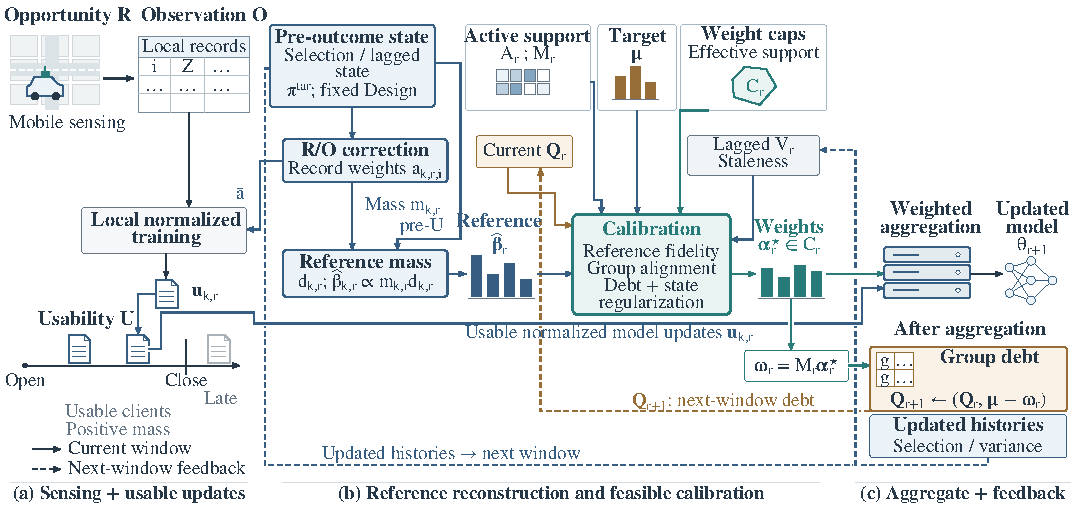
\includegraphics[width=\textwidth]{fig1_raven_problem_framework.pdf}
\caption{RAVEN-MCS workflow. (a)~Opportunity/observation correction supplies normalized
local weights and reference mass; raw records remain local.
(b)~Pre-$U$ correction forms $\widehat{\boldsymbol\beta}_r$; calibration produces
feasible $\boldsymbol\alpha_r^\star$ from current support, composition, target,
and state. Exact target matching need not be feasible.
(c)~Weighted updates are aggregated before debt/history updates.
Solid/dashed arrows denote current-window flow/next-window feedback.
Carriers and vectors are schematic.}
\label{fig:raven_overview}
\end{figure*}

\subsection{Windowed Asynchronous Mobile Crowdsensing}
\label{subsec:windowed_mcs}

A server coordinates clients $\mathcal K=\{1,\ldots,K\}$ over atomic units
$i=(n,t)\in\mathcal I$, with spatial index $n$, absolute time $t$, target
$Y_i\in\mathcal Y\subseteq\mathbb R$, and label-free deployment context
$C_i^{\mathrm{dep}}$.  The target is revealed only if observed, with client
measurement $Z_{k,r,i}$ in window $r$.  Clients train one completion predictor
$f_\theta$, $\theta\in\Theta\subseteq\mathbb R^d$, producing
$\widehat Y_i=f_\theta(i;C_i^{\mathrm{dep}})\in\mathcal Y$.

The server holds $\theta_r$ fixed throughout
$\mathcal W_r=[T_r,T_{r+1})$.  Client $k$ may start from an older model
$\theta_{\sigma_{k,r}}$, $\sigma_{k,r}\le r$, with model-version staleness
$\tau_{k,r}=r-\sigma_{k,r}$.  At close, the server determines usable attempts
and performs one aggregation transition $\theta_r\to\theta_{r+1}$.
Individual arrivals do not trigger updates as in immediate-update FedAsync.
Comparisons freeze exogenous mobile/update events across methods without
assuming independence. Training and delivery are asynchronous; window-close
aggregation jointly weights usable clients.

\subsection{Two-Stage, Three-Layer Non-Random Selection}
\label{subsec:selection_process}

The sensing stage comprises opportunity $R$ and observation $O$, followed by
update usability $U$.  The indicator $R_{k,r,i}\in\{0,1\}$ places $(k,i)$ in
the opportunity/risk set before sensing.  Conditional on $R_{k,r,i}=1$,
$O_{k,r,i}\in\{0,1\}$ records observation.  A nonempty observed buffer
registers a client in $\mathcal E_r$.  Its attempt has $U_{k,r}=1$ only if
computation and transmission succeed by $T_{r+1}$ with
$\tau_{k,r}\le S_{\max}$, the frozen admissible staleness.  Failed attempts
remain logged as $U_{k,r}=0$.  The usable set is
$\mathcal U_r=\{k\in\mathcal E_r:U_{k,r}=1\}$.  Removing zero-mass clients in
Section~\ref{sec:reconstruction} yields the aggregation set
$\mathcal A_r\subseteq\mathcal U_r$.
Usability is shared within an attempt; opportunity and observation are
unit-specific. Registration, usability, and positive mass define distinct sets.

The label-free maps $h:\mathcal I\to\mathcal G$ and
$s:\mathcal I\to\mathcal S$ specify deployment groups and opportunity strata.
The former defines the mass to be served, whereas the latter pools mobile exposure for
selection modeling.  They need not coincide and are frozen from public or
training-side information without test labels.  The normalized opportunity law is
\begin{equation}
 P_r^{\mathrm{opp}}(k,i)
 =
 \pi^{\mathrm{opp}}_{k,s(i),r}
 \nu^{\mathrm{opp}}_{k,r}(i\mid s(i)),
 \qquad
 \sum_{k,i}P_r^{\mathrm{opp}}(k,i)=1,
 \label{eq:opp_event_law}
\end{equation}
Here $\pi^{\mathrm{opp}}_{k,s,r}$ is client--stratum opportunity mass and
$\nu^{\mathrm{opp}}_{k,r}(i\mid s)$ is its conditional atomic law.  The
realized indicators $R_{k,r,i}$ record events from this process; they are not
mutually independent Bernoulli draws.  Subsequent selection probabilities are
\begin{align}
 p^{\mathrm{obs}}_{k,r,i}
 &\triangleq
 \Pr\!\left(
 O_{k,r,i}=1
 \mid
 R_{k,r,i}=1,\mathcal{H}^{\mathrm{obs}}_{k,r,i}
 \right),
 \label{eq:pobs_def}\\
 q^{\mathrm{use}}_{k,r}
 &\triangleq
 \Pr\!\left(
 U_{k,r}=1
 \mid
 k\in\mathcal{E}_r,\mathcal{H}^{\mathrm{use}}_{k,r}
 \right).
 \label{eq:quse_def}
\end{align}
The history $\mathcal H^{\mathrm{obs}}_{k,r,i}$ contains only information
available before $O_{k,r,i}$.  The pre-$U$ history
$\mathcal H^{\mathrm{use}}_{k,r}$ may include the already realized sensing-side
registration state, but excludes the realized computation/transmission outcome,
future events, and the current update vector to be weighted.  The opportunity law describes how sensing units enter risk sets, not which
responses are subsequently observed.  A target group can span several
opportunity strata, so its desired mass cannot be substituted for a stratum's
selection probability.

\subsection{Public Deployment Target and Compatible Target Measures}
\label{subsec:target_measures}

The public atomic target on $\mathcal I_{\mathrm{dep}}\subseteq\mathcal I$ is
\begin{equation}
    \varpi_i^{\mathrm{tar}}\ge0,
    \qquad
    \sum_{i\in\mathcal{I}_{\mathrm{dep}}}
    \varpi_i^{\mathrm{tar}}=1.
    \label{eq:atomic_target}
\end{equation}
Its deployment-group marginal is
$\mu_g=\sum_{i:h(i)=g}\varpi_i^{\mathrm{tar}}$, with
$\boldsymbol\mu\in\Delta^{|\mathcal G|-1}$.  Opportunity correction uses a
compatible client--atomic target $\pi^{\mathrm{tar}}_{k,i}$, whose
client--stratum marginal is
$\pi^{\mathrm{tar}}_{k,s}=\sum_{i:s(i)=s}\pi^{\mathrm{tar}}_{k,i}$.
Compatibility requires
\begin{equation}
    \sum_k\pi^{\mathrm{tar}}_{k,i}
    =
    \varpi_i^{\mathrm{tar}},
    \qquad
    \sum_{k,s}\pi^{\mathrm{tar}}_{k,s}=1.
    \label{eq:target_compatibility}
\end{equation}
The atomic target fixes sensing-unit importance; its compatible client
allocation and stratum marginal supply the reference for corrected
client-mass estimates.
\appreffull{app:deferred_constructions} of the separate Supplementary Material uses public
client shares and conditional atomic target masses, all frozen before
test-label evaluation.  Design is configured before each window and fixed
within it, as specified in Section~\ref{subsec:global_update}.

\subsection{Deployment-Target Risk Versus Arrival Risk}
\label{subsec:target_risk}

For squared loss $\ell(\widehat Y,Y)=\tfrac12(\widehat Y-Y)^2$, define
\begin{equation}
 \mathcal{R}_{\mu}(\theta)
 =
 \sum_{i\in\mathcal{I}_{\mathrm{dep}}}
 \varpi_i^{\mathrm{tar}}
 \ell\!\left(
 f_{\theta}(i;C_i^{\mathrm{dep}}),Y_i
 \right).
 \label{eq:target_risk}
\end{equation}
Quantities without a window index below denote frozen evaluation-period
marginals of the corresponding pre-outcome mechanisms.  The sequential
inclusion law is $P^{\mathrm{opp}}(k,i)p^{\mathrm{obs}}_{k,i}q^{\mathrm{use}}_k$.
The label-free arrival intensity is estimated by
\begin{equation}
 \widehat r_i^{\mathrm{arr}}
 =
 \sum_k
 \widehat\pi^{\mathrm{opp}}_{k,s(i)}
 \widehat\nu^{\mathrm{opp}}_{k}(i\mid s(i))
 \widehat p^{\mathrm{obs}}_{k,i}
 \widehat q^{\mathrm{use}}_{k,s(i)},
 \label{eq:arrival_intensity}
\end{equation}
Here $\widehat q^{\mathrm{use}}_{k,s}$ is the evaluation-period marginal of
the legal pre-$U$ model over registered attempts associated with stratum $s$,
not a probability conditioned on the realized delivery outcome.  Normalize
\begin{equation}
 \widetilde\rho_i^{\mathrm{arr}}
 =
 \frac{\widehat r_i^{\mathrm{arr}}}
 {\sum_{j\in\mathcal{I}_{\mathrm{dep}}}\widehat r_j^{\mathrm{arr}}},
 \label{eq:arrival_distribution}
\end{equation}
and define
\begin{equation}
 \mathcal{R}_{\rho}(\theta)
 =
 \sum_{i\in\mathcal{I}_{\mathrm{dep}}}
 \widetilde\rho_i^{\mathrm{arr}}
 \ell\!\left(
 f_{\theta}(i;C_i^{\mathrm{dep}}),Y_i
 \right).
 \label{eq:arrival_risk}
\end{equation}
Both risks evaluate the same deployment units under different weighting laws
and can coincide for a fixed predictor. The plug-in arrival law pools
evaluation-period marginals; it does not replace the attempt-level conditional
usability probabilities used for training-time correction.

\subsection{Structural Alignment Objective}
\label{subsec:design_objective}

Let $\mathbf c^g_{k,r}\in\Delta^{|\mathcal G|-1}$ and
$\mathbf c^s_{k,r}\in\Delta^{|\mathcal S|-1}$ denote corrected within-client
group and stratum compositions, constructed in Section~\ref{sec:reconstruction}.
With $M_r=[\mathbf c^g_{k,r}]_{k\in\mathcal A_r}$, weights
$\boldsymbol\alpha_r\in\mathcal C_r$ produce group composition
$\boldsymbol\omega_r=M_r\boldsymbol\alpha_r$.
Section~\ref{sec:calibration} defines the feasible calibration weights.

For server step size $\eta_r>0$, let
$I_r=\mathbf1\{|\mathcal A_r|>0\}$ and
$S_R=\sum_{r=0}^{R-1}\eta_r I_r$.  All prefix averages below require $S_R>0$:
\begin{equation}
    \overline{\boldsymbol\omega}_R
    =
    \frac{1}{S_R}
    \sum_{r=0}^{R-1}
    \eta_r I_r\boldsymbol\omega_r.
    \label{eq:omega_bar}
\end{equation}
The group mismatch is
$\Delta_{\mathrm{group}}(R)=\|\overline{\boldsymbol\omega}_R-\boldsymbol\mu\|_1$.
Step-weighted active-window averaging matches debt's update scale rather than
wall time.
Extend $\alpha_{k,r}=0$ to inactive clients $k\notin\mathcal A_r$ and define
\begin{equation}
 \widehat\Pi_{k,s}(R)
 =
 \frac{1}{S_R}
 \sum_{r=0}^{R-1}
 \eta_r I_r\,
 \alpha_{k,r}\,
 c^{s}_{k,r,s}.
 \label{eq:Pi_hat_ks}
\end{equation}
\begin{equation}
 \Delta_{c\text{-}s}(R)
 =
 \sum_{k,s}
 \left|
 \widehat\Pi_{k,s}(R)-\pi^{\mathrm{tar}}_{k,s}
 \right|.
 \label{eq:delta_cs}
\end{equation}
Normalization gives $\sum_{k,s}\widehat\Pi_{k,s}(R)=1$.  Both structural
distances lie in $[0,2]$. Their corresponding total-variation distances are
$\Delta/2$; a change of $\delta$ in either $L_1$ distance is therefore
$50\delta$ percentage points of total variation.  The Uniform benchmark, same-support hindsight comparison,
and practical equivalence convention are specified in
Section~\ref{subsec:equivalence_band}.

\FloatBarrier
\section{Selection-Layer-Aware Target Reconstruction}
\label{sec:reconstruction}

Sequential IPW and H\'ajek normalization connect within-client training weights
to an estimated, stabilized between-client mass reference.

\subsection{Opportunity/Design Correction}
\label{subsec:design_correction}

The ideal opportunity ratio on target-supported client--atomic pairs is
\begin{equation}
 \zeta^{o}_{k,r,i}
 =
 \frac{\pi^{\mathrm{tar}}_{k,s(i)}}
      {\pi^{\mathrm{opp}}_{k,s(i),r}}
 \frac{\nu^{\mathrm{tar}}_{i\mid s(i)}}
      {\nu^{\mathrm{opp}}_{k,r}(i\mid s(i))}
 =
 \frac{\pi^{\mathrm{tar}}_{k,i}}
      {P_r^{\mathrm{opp}}(k,i)}.
 \label{eq:design_ratio_general}
\end{equation}
Within-stratum exchangeability,
$\nu^{\mathrm{opp}}_{k,r}(i\mid s)=\nu^{\mathrm{tar}}_{i\mid s}$,
cancels the conditional atomic ratio.  The implementation estimates the
remaining opportunity mass from lagged history and floors its denominator:
\begin{equation}
 \widehat\zeta^{o}_{k,r,s}
 =
 \frac{\pi^{\mathrm{tar}}_{k,s}}
 {\max\{\widehat\pi^{\mathrm{opp}}_{k,s,r},\pi_{\min}\}}.
 \label{eq:design_ratio_simple}
\end{equation}
One admissible smoothed count estimator is
\begin{align*}
 C^{\mathrm{opp}}_{k,s,r}
 &=
 \rho_{\mathrm{opp}}C^{\mathrm{opp}}_{k,s,r-1}
 +N^{\mathrm{opp}}_{k,s,r-1},\\
 \widehat\pi^{\mathrm{opp}}_{k,s,r}
 &=
 \frac{C^{\mathrm{opp}}_{k,s,r}+\epsilon_{\mathrm{opp}}}
 {\sum_{j,u}
 (C^{\mathrm{opp}}_{j,u,r}+\epsilon_{\mathrm{opp}})}.
\end{align*}
Under \eqref{eq:design_factor}, Design on uses this ratio.  Off sets it to one
and retains the opportunity arrival law.  Both are configured before opening
and fixed within the window.

\subsection{Observation Correction and Local H\'ajek Normalization}
\label{subsec:observation_hajek}

For ideal weight $a^\star_{k,r,i}=\zeta^o_{k,r,i}/p^{\mathrm{obs}}_{k,r,i}$,
the stabilized plug-in and corrected masses are
\begin{equation}
 a_{k,r,i}
 =
 \min\!\left\{
 a_{\max},
 \frac{\widehat\zeta^{o}_{k,r,i}}
 {\max\{\widehat p^{\mathrm{obs}}_{k,r,i},p_{\min}\}}
 \right\}.
 \label{eq:a_stabilized}
\end{equation}
\begin{align}
m_{k,r}
    &=
    \sum_i
    R_{k,r,i}O_{k,r,i}a_{k,r,i},
    \label{eq:m_total}\\
m^{g}_{k,r,g}
 &=
 \sum_i
 R_{k,r,i}O_{k,r,i}a_{k,r,i}
 \mathbf{1}\{h(i)=g\},
 \label{eq:m_group}\\
m^{s}_{k,r,s}
 &=
 \sum_i
 R_{k,r,i}O_{k,r,i}a_{k,r,i}
 \mathbf{1}\{s(i)=s\}.
 \label{eq:m_stratum}
\end{align}
Only $\mathcal A_r=\{k\in\mathcal U_r:m_{k,r}>0\}$ is aggregated.  Define
$\overline a_{k,r,i}=R_{k,r,i}O_{k,r,i}a_{k,r,i}/m_{k,r}$,
$c^g_{k,r,g}=m^g_{k,r,g}/m_{k,r}$, and
$c^s_{k,r,s}=m^s_{k,r,s}/m_{k,r}$.  These record weights and compositions
normalize within each active client.  Local ESS,
\begin{equation}
 n^{\mathrm{eff}}_{k,r}
 =
 \frac{m_{k,r}^2}
 {\sum_i
  (R_{k,r,i}O_{k,r,i}a_{k,r,i})^2}
 =
 \frac{1}{\sum_i\overline a_{k,r,i}^2}.
 \label{eq:neff}
\end{equation}
measures concentration, not corrected target mass $m_{k,r}$.
Training uses the normalized objective
\begin{equation}
 \widehat F^{H}_{k,r}(\theta)
 =
 \sum_i
 \overline a_{k,r,i}
 \frac{1}{2}
 \left(
 f_{\theta}(i;C_i^{\mathrm{dep}})
 -
 Z_{k,r,i}
 \right)^2.
 \label{eq:local_hajek_objective}
\end{equation}
Starting at $\theta_{\sigma_{k,r}}$, the client takes $E_{\mathrm{loc}}$ steps
on $\widehat F^H_{k,r}$ with step size $\gamma_r>0$, producing normalized
displacement
\begin{equation}
 \mathbf{u}_{k,r}
 =
 \frac{
 \theta_{\sigma_{k,r}}
 -
 \theta^{(E_{\mathrm{loc}})}_{k,r}
 }{\gamma_r E_{\mathrm{loc}}}.
 \label{eq:normalized_update}
\end{equation}
This divides out the explicit local learning-rate and step-count factors;
the training path still determines the displacement.  Constant within-client correction cancels during
normalization.  Heterogeneous propensities supply different inputs, although
clipping can still equalize realized weights.
\appref{app:local_hajek} derives this cancellation.

\subsection{Usable-Update Correction and Reference Aggregation Mass}
\label{subsec:usable_correction}

For $k\in\mathcal A_r$, the pre-$U$ estimate gives
\begin{equation}
 d_{k,r}
 =
 \min\!\left\{
 d_{\max},
 \frac{1}
 {\max\{\widehat q^{\mathrm{use}}_{k,r},q_{\min}\}}
 \right\},
 \label{eq:d_use}
\end{equation}
Set $b_{k,r}=m_{k,r}d_{k,r}$ and normalize:
\begin{equation}
 \widehat\beta_{k,r}
 =
 \frac{b_{k,r}}
 {\sum_{j\in\mathcal{A}_r}b_{j,r}},
 \qquad
 k\in\mathcal{A}_r.
 \label{eq:beta_ref}
\end{equation}
Local H\'ajek normalization removes total mass from the local objective;
$m_{k,r}d_{k,r}$ preserves relative corrected mass and accounts for
usable-update selection at the server.
\appref{app:ideal_factorization} gives the ideal untruncated
$\beta^\star\overline a^\star$ factorization. The stabilized reference
$\widehat{\boldsymbol\beta}_r$ is distinct from the feasible decision
$\boldsymbol\alpha_r$: incomplete support can prevent
$M_r\widehat{\boldsymbol\beta}_r=\boldsymbol\mu$.
Section~\ref{sec:calibration} calibrates this reference.

\subsection{Information Boundary and Stabilization}
\label{subsec:information_boundary}

Opportunity estimates are lagged, observation models exclude current responses,
and usable-update models exclude $U$ outcomes and future information.  Current
update coordinates, norms, or directions never determine that update's weight.
Clipping stabilizes finite samples but introduces error distinct from
estimation error.  Ideal recovery requires support, correct ratios, and
sequential identification (Section~\ref{sec:theory}).  Inactive clipping alone
does not establish these conditions.

\section{Feasibility-Aware Target Calibration}
\label{sec:calibration}

Calibration balances reference fidelity, target composition, and accumulated
under-service on available clients.

\subsection{Feasible Aggregation Set}
\label{subsec:feasible_set}

For $K_r=|\mathcal A_r|>0$, choose $\boldsymbol\alpha_r\in\mathbb R^{K_r}$ in
\begin{equation}
 \mathcal{C}_r
 =
 \left\{
 \boldsymbol\alpha:
 \mathbf{1}^{\top}\boldsymbol\alpha=1,\;
 0\le\alpha_k\le\overline\alpha_r,\;
 \|\boldsymbol\alpha\|_2^2\le\frac{1}{\overline E_r}
 \right\},
 \label{eq:Cr}
\end{equation}
The cap $\overline\alpha_r=\min\{1,\max\{\alpha_{\max},1/K_r\}\}$ and
support bound $\overline E_r=\min\{E_{\min},K_r\}$ use frozen
$0<\alpha_{\max}\le1$, $E_{\min}\ge1$ (\appref{app:correction_constraints}).
These definitions make Uniform feasible while controlling single-client
dominance and minimum effective support.  The reconstructed reference need not
satisfy these constraints.  The lagged variance proxy is
\begin{equation}
 v_{k,r}
 =
 \frac{
 \overline S_{k,r^-}^{\,2}
 }{
 \max\{n^{\mathrm{eff}}_{k,r},1\}
 }
 +
 v_{\mathrm{floor}},
 \qquad
 V_r=\operatorname{diag}(v_{k,r})\succeq0,
 \label{eq:variance_proxy}
\end{equation}
This lagged proxy, rather than true update variance, and frozen staleness
$\overline{\boldsymbol\tau}_r\ge0$ are available before weighting without
inspecting the current update vector.

\subsection{Long-Term Target Debt}
\label{subsec:debt}

Initialize $\mathbf Q_0=\mathbf0$.  In active windows, accumulated group
under-service follows
$\mathbf Q_{r+1}=[\mathbf Q_r+\eta_r(\boldsymbol\mu-\boldsymbol\omega_r)]_+$,
where $\boldsymbol\omega_r=M_r\boldsymbol\alpha_r$.  Inactive windows leave
debt unchanged.
For effective step mass $S_R=\sum_{r<R}\eta_r I_r>0$,
the deterministic accounting bound is
\begin{equation}
 \left\|
 \overline{\boldsymbol\omega}_R-\boldsymbol\mu
 \right\|_1
 \le
 \frac{
 2\|\mathbf{Q}_R\|_1
 }{S_R}.
 \label{eq:debt_bound}
\end{equation}
\begin{proof}
Coordinatewise summation bounds the positive part of cumulative signed
under-service by $\mathbf Q_R$. The signed under-service vector sums to zero,
so its $\ell_1$ norm equals twice its positive mass (\appref{app:proof_debt_bound}).
\end{proof}
A vanishing bound requires $\|\mathbf Q_R\|_1=o(S_R)$.

\subsection{Feasibility-Aware Calibration Program}
\label{subsec:P2}

Each active window solves
$\min_{\boldsymbol\alpha\in\mathcal C_r}J_r(\boldsymbol\alpha)$:
\begin{align}
 J_r(\boldsymbol\alpha)
 ={}&-\mathbf{Q}_r^{\top}M_r\boldsymbol\alpha
 +\frac{\lambda_g}{2}
 \|M_r\boldsymbol\alpha-\boldsymbol\mu\|_2^2
 \nonumber\\
 &+\frac{\lambda_{\beta}}{2}
 \|\boldsymbol\alpha-\widehat{\boldsymbol\beta}_r\|_2^2
 \nonumber\\
 &+\frac{\lambda_v}{2}
 \boldsymbol\alpha^{\top}V_r\boldsymbol\alpha
 +\lambda_s\overline{\boldsymbol\tau}_r^{\top}\boldsymbol\alpha.
\label{eq:P2_objective}
\end{align}
The anchor controls client-weight departures from the reference; the group
term matches deployment composition in a different space. Debt prioritizes
accumulated under-service, while variance and staleness use their defined
proxies. Theorem~\ref{thm:calibration} concerns the exact program.

\subsection{Global Update and Window Logic}
\label{subsec:global_update}

With the calibration solution $\boldsymbol\alpha_r^\star$, aggregate the normalized updates
of \eqref{eq:normalized_update}:
\begin{equation}
 \theta_{r+1}
 =
 \theta_r
 -
 \eta_r
 \sum_{k\in\mathcal{A}_r}
 \alpha^\star_{k,r}\mathbf{u}_{k,r}.
 \label{eq:server_update}
\end{equation}
The order is reference reconstruction, calibration, aggregation, then debt
(Section~\ref{subsec:debt}) and lagged-state updates.
If $\mathcal A_r=\varnothing$, carry forward model and debt without adding
the window to $S_R$.

The recorded configuration $D_t\in\{\mathrm{on},\mathrm{off}\}$ is fixed before
opening and throughout window $t$:
\begin{equation}
\widehat\zeta^{o}_{k,t,i}
=
\begin{cases}
\dfrac{\pi^{\mathrm{tar}}_{k,s(i)}}
{\max\{\widehat\pi^{\mathrm{opp}}_{k,t,s(i)},\pi_{\min}\}}, & D_t=\mathrm{on},\\[1.5mm]
1, & D_t=\mathrm{off}.
\end{cases}
\label{eq:design_factor}
\end{equation}
RAVEN abbreviates RAVEN-MCS. RAVEN-Design fixes Design on throughout a run,
applying the lagged ratio in \eqref{eq:design_factor}; RAVEN-NoDesign fixes it
off, setting the ratio to one and retaining the opportunity arrival law.
Other correction, calibration, and debt-update steps coincide. The catalogue check
\eqref{eq:design_gate} can inform configuration only when its catalogue and
public lookup already exist before opening, independently of coverage.

\begin{algorithm}[t]
\caption{Window-close RAVEN-MCS with configured Design}
\label{alg:window_close}
\begin{algorithmic}[1]
\REQUIRE window $t$; recorded $R,O,U$; model $\theta_t$ and debt $\mathbf Q_t$;
public $\boldsymbol\mu,\pi^{\mathrm{tar}}$; pre-window $D_t$ and frozen
correction/constraint parameters, $\eta_t$, and lagged states
\ENSURE $\theta_{t+1}$, $\mathbf Q_{t+1}$
\STATE Form $\mathcal E_t$ and $\mathcal U_t=\{k\in\mathcal E_t:U_{k,t}=1\}$.
\STATE Apply configured Design via \eqref{eq:design_factor}.
\STATE Compute $a_{k,t,i}$ and $m_{k,t}$ via \eqref{eq:a_stabilized}--\eqref{eq:m_total};
set $\mathcal A_t=\{k\in\mathcal U_t:m_{k,t}>0\}$.
\IF{$\mathcal A_t=\varnothing$}
\STATE Carry forward $\theta_t,\mathbf Q_t$; exclude this window from $S_R$; stop this window.
\ELSE
\STATE Reconstruct $d_{k,t}$ and $\widehat{\boldsymbol\beta}_t$ via
\eqref{eq:d_use}--\eqref{eq:beta_ref}.
\STATE Form $\mathcal C_t$ and lagged $V_t,\overline{\boldsymbol\tau}_t$;
solve the calibration program for $\boldsymbol\alpha_t^\star$.
\STATE Update $\theta_{t+1}$ by \eqref{eq:server_update}.
\STATE Set $\boldsymbol\omega_t=M_t\boldsymbol\alpha_t^\star$;
apply the debt recursion of Section~\ref{subsec:debt}.
\STATE Advance lagged selection and variance states.
\ENDIF
\end{algorithmic}
\end{algorithm}

\subsection{Aggregate Opportunity-Coverage Diagnostic}
\label{subsec:agg_certificate_alg}
\label{subsec:agg_coverage_object}

For target-positive pairs $I_{\mathrm{tar}}=\{(k,s):\pi^{\mathrm{tar}}_{k,s}>0\}$,
diagnose realized coverage
\begin{equation}
 C_t
 =
 \sum_{(k,s)\in I_{\mathrm{tar}}}
 \pi^{\mathrm{tar}}_{k,s}
 \,
 \mathbf{1}\!\left\{\pi^{\mathrm{opp}}_{k,s,t}\ge\pi_{\mathrm{safe}}\right\},
 \label{eq:agg_Ct}
\end{equation}
Here $\pi^{\mathrm{opp}}_{k,s,t}$ is lagged opportunity mass and
$\pi_{\mathrm{safe}}$ is frozen.  Lookup construction is in
\appref{app:itar_lookup}.  Unlike conformal prediction
sets~\cite{lu2023federated,plassier2023conformal}, this is aggregate opportunity
coverage.  The diagnostic uses pre-window information $F_{t-}$ and
\begin{equation}
 k_n=\lceil(n+1)(1-\alpha)\rceil,
 \qquad
 \alpha=0.05,
 \label{eq:agg_kn}
\end{equation}
Use the historical same-block quantile $q_t=S^{\mathrm{cal}}_{(k_n)}$ in
\begin{equation}
 C^{\mathrm{LCB}}_t=\max\{0,\widehat C_t-q_t\},
 \label{eq:agg_CLCB}
\end{equation}
with $\mathrm{Gate}_t=\mathbf1\{C_t^{\mathrm{LCB}}\ge\tau_{\mathrm{cov}}\}$,
$\tau_{\mathrm{cov}}=0.05$.  WARMUP/RESET set Gate to zero without switching
Design.  Prediction and calibration use completed past windows.  Realized $C_t$
evaluates the bound and updates diagnostic state only after completion.
Section~\ref{subsec:agg_coverage_theory} gives conditional guarantees.  The
supplemental algorithm specifies the historical quantile construction.

\section{Theoretical Analysis}
\label{sec:theory}

\subsection{Assumptions}
\label{subsec:assumptions}

\noindent\textbf{A1 (Compatible target support and positivity).}
Public targets satisfy \eqref{eq:atomic_target} and
\eqref{eq:target_compatibility}.  Inverse factors are applied only where
$P_r^{\mathrm{opp}}$, $p^{\mathrm{obs}}$, and $q^{\mathrm{use}}$ are
strictly positive on target-supported events.

\noindent\textbf{A2 (Sequential pre-outcome ignorability).}
Conditional on the legal history at each stage, $O$ and $U$ are
conditionally mean-ignorable for the reconstructed moment.  The $O$ model
uses only $\mathcal{H}^{\mathrm{obs}}$; the $U$ model may use the realized
sensing-side registration state, but not the future $U$ outcome
(display in the supplemental material).

\noindent\textbf{A3 (Correct ideal ratios and cluster-level regularity).}
The ideal estimator uses correct population ratios without clipping.
As $N_R^{\mathrm{opp}}\rightarrow\infty$,
weighted cluster sums obey a weak law and the H\'ajek denominator stays
strictly positive.

\noindent\textbf{A4 (Convex calibration).}
In every active window, $K_r\ge1$, $0<\alpha_{\max}\le1$, $E_{\min}\ge1$,
$V_r\succeq0$, $\lambda_{\beta}>0$, and
$\lambda_g,\lambda_v,\lambda_s\ge0$.  The feasible set is \eqref{eq:Cr}.

\noindent\textbf{A5 (Positivity and shared support).}
All target-supported events entering the estimator on $\mathcal A_r$ have
positive opportunity, observation, and usable-update margins.  The ideal and
the practical reference share $\mathcal{A}_r$, $M_r$, and $\mathcal{C}_r$,
and the unnormalized H\'ajek mass obeys
$\mathbf{1}^{\top}b\ge B_{\min}>0$.  To retain this shared support under
Design off, RAVEN-NoDesign fixes $\widehat\zeta=1$ on
$\{\pi^{\mathrm{tar}}=0\}$ as well.

\noindent\textbf{A6a (Inactive stabilization at the true margins).}
On A5's active support the true margins clear every stabilizer of
\eqref{eq:design_ratio_simple}, \eqref{eq:a_stabilized}, and \eqref{eq:d_use}:
$\pi^{\mathrm{opp}}\ge\pi_{\min}$, $p^{\mathrm{obs}}\ge p_{\min}$,
$\pi^{\mathrm{tar}}/(\pi^{\mathrm{opp}}p^{\mathrm{obs}})\le a_{\max}$ with
Design on and $1/p^{\mathrm{obs}}\le a_{\max}$ with Design off, and
$1/q^{\mathrm{use}}\le d_{\max}$; when $d_{\max}\le1/q_{\min}$, as for the
frozen constants, the last clause also gives $q^{\mathrm{use}}\ge q_{\min}$.
A6a ensures that the map returns the ideal untruncated ratios and is sufficient
for the stabilization error in \eqref{eq:eps_stab} to vanish.

\noindent\textbf{A6b (Bounded interpolation error).}
On A5's active support the pre-outcome estimates satisfy
$|\widehat\pi^{\mathrm{opp}}-\pi^{\mathrm{opp}}|\le\varepsilon_\pi$,
$|\widehat p^{\mathrm{obs}}-p^{\mathrm{obs}}|\le\varepsilon_p$, and
$|\widehat q^{\mathrm{use}}-q^{\mathrm{use}}|\le\varepsilon_q$.

\subsection{Target Risk Is Not Arrival Risk}
\label{subsec:prop_risk}

\begin{proposition}[Target-vs-arrival risk distinction]
\label{prop:risk}
Distinct normalized laws $\boldsymbol\varpi^{\mathrm{tar}}$ and
$\widetilde{\boldsymbol\rho}^{\mathrm{arr}}$ on the same finite supported
domain admit a bounded nonnegative error profile $e_i$ with
\begin{equation}
 \sum_i
 \varpi_i^{\mathrm{tar}}e_i
 \neq
 \sum_i
 \widetilde\rho_i^{\mathrm{arr}}e_i.
 \label{eq:prop1_nonidentity}
\end{equation}
Equality for every bounded profile implies equal laws.
\end{proposition}

\begin{proof}
Let $d_i=\varpi_i^{\mathrm{tar}}-\widetilde\rho_i^{\mathrm{arr}}$ and
$e_i=\mathbf1\{d_i>0\}$. Normalization gives $\sum_i d_i=0$, hence
$\sum_i d_i e_i>0$; coordinate indicators prove the converse
(\appref{app:proof_prop1}).
\end{proof}
A fixed predictor may nevertheless have equal risks.

\subsection{Normalized Sequential Target Reconstruction}
\label{subsec:prop_reconstruction}

Let $\mathcal O_r$ be the multiset of opportunity events, with marks
$(k_e,i_e)$ distributed by \eqref{eq:opp_event_law}.  Sequential selection gives
\begin{equation}
 \chi_e
 =
 O_e U_{k_e,r}
 \frac{
 \pi^{\mathrm{tar}}_{k_e,i_e}
 }{
 P_r^{\mathrm{opp}}(k_e,i_e)
 p^{\mathrm{obs}}_{k_e,r,i_e}
 q^{\mathrm{use}}_{k_e,r}
 }.
 \label{eq:chi_event}
\end{equation}

\begin{proposition}[Normalized target reconstruction]
\label{prop:reconstruction}
Under A1--A3, for any bounded test function $\psi(k,i)$ distinct from the
Design factor of \eqref{eq:design_factor},
\begin{equation}
 \widehat\Phi_R
 =
 \frac{
 \sum_{r<R}
 \sum_{e\in\mathcal{O}_r}
 \chi_e\psi(k_e,i_e)
 }{
 \sum_{r<R}
 \sum_{e\in\mathcal{O}_r}
 \chi_e
 }
 \xrightarrow{p}
 \Phi^{\mathrm{tar}},
 \label{eq:hajek_phi}
\end{equation}
where
\begin{equation}
 \Phi^{\mathrm{tar}}
 =
 \sum_{k,i}
 \pi^{\mathrm{tar}}_{k,i}\psi(k,i).
 \label{eq:target_phi}
\end{equation}
Client--stratum indicators recover $\pi^{\mathrm{tar}}_{k,s}$; compatibility
\eqref{eq:target_compatibility} makes group indicators recover $\mu_g$.
\end{proposition}

\begin{proof}
Sequential conditional expectations cancel $O/U$ factors; opportunity
integration cancels $P_r^{\mathrm{opp}}$. Under A1--A3, the cluster weak law
gives numerator and denominator limits $\Phi^{\mathrm{tar}}$ and $1$ per opportunity
event, yielding the pooled ratio limit. Proof details: \appref{app:proof_prop2}.
\end{proof}
Pooled consistency does not imply finite-window realizability.

\subsection{Existence and Uniqueness of Feasible Calibration}
\label{subsec:theorem_calibration}

\begin{theorem}[Unique solution of the calibration program]
\label{thm:calibration}
Under A4, every active window has a nonempty compact convex feasible set
$\mathcal{C}_r$, and the calibration program
$\min_{\boldsymbol\alpha\in\mathcal{C}_r}J_r(\boldsymbol\alpha)$
has a unique global minimizer $\boldsymbol\alpha_r^\star$.
\end{theorem}

\begin{proof}
Uniform satisfies \eqref{eq:Cr}, ensuring nonemptiness. The constrained simplex
is compact and convex; continuity and the Hessian bound
$\nabla^2J_r\succeq\lambda_\beta I\succ0$ give existence and uniqueness under A4
(\appref{app:proof_theorem1}).
\end{proof}

\subsection{Practical Plug-in Perturbation}
\label{subsec:prop_plugin}

Let $\mathcal T$ combine \eqref{eq:design_ratio_simple},
\eqref{eq:a_stabilized}, \eqref{eq:d_use}, and \eqref{eq:beta_ref}.
Its reference at true margins on $\mathcal A_r$ is
$\boldsymbol\beta_r^{\mathcal T}$; relative to ideal untruncated
$\boldsymbol\beta_r^\star$, stabilization error is
\begin{equation}
\varepsilon_{\mathrm{stab},r}
=
\bigl\|\boldsymbol\beta_r^{\mathcal T}-\boldsymbol\beta_r^\star\bigr\|_1 .
\label{eq:eps_stab}
\end{equation}
Write $n_r=\max_{k\in\mathcal A_r}\sum_iR_{k,r,i}O_{k,r,i}$ and
$K_r=|\mathcal A_r|$.

\begin{proposition}[Practical plug-in perturbation]
\label{prop:practical_plugin}
Assume A1, A4, A5, and A6b.  Let the stabilized window mass obey
$\mathbf{1}^{\top}b_r^{\mathcal T}\ge B_{\min}>0$ at the true margins, and let
the ideal and the implemented reference share $\mathcal{A}_r$, $M_r$, and
$\mathcal{C}_r$.  Write $\boldsymbol\beta_r^\star$ for the same-window ideal reference,
$\widehat{\boldsymbol\beta}_r$ for the implemented clipped plug-in, and
$\boldsymbol\alpha^\star(\boldsymbol\beta)$ for the unique calibration minimizer
at the fixed state.  Then
\begin{align}
\bigl\|\widehat{\boldsymbol\beta}_r-\boldsymbol\beta_r^\star\bigr\|_1
&\le
C_1\bigl(\varepsilon_\pi+\varepsilon_p+\varepsilon_q\bigr)
+\varepsilon_{\mathrm{stab},r},
\label{eq:g4_beta}\\
\bigl\|\widehat{\boldsymbol\alpha}_r-\boldsymbol\alpha_r^\star\bigr\|_2
&\le
\bigl\|\widehat{\boldsymbol\beta}_r-\boldsymbol\beta_r^\star\bigr\|_2,
\label{eq:g4_alpha}\\
\bigl\|M_r(\widehat{\boldsymbol\alpha}_r-\boldsymbol\alpha_r^\star)\bigr\|_2
&\le
\|M_r\|_2\,
\bigl\|\widehat{\boldsymbol\beta}_r-\boldsymbol\beta_r^\star\bigr\|_2,
\label{eq:g4_comp}
\end{align}
Here $C_1$ and its Design-on/off constants are defined in
\eqref{eq:g4_c1}.  On the shared fixed state, the bounds hold without A6a, which is sufficient
for $\varepsilon_{\mathrm{stab},r}=0$ but not necessary when normalization
cancels distortions. The worst-case envelope can be loose:
the frozen Design-on constants give $L_\pi\le2\times10^{13}$.
\end{proposition}

\begin{proof}
Lipschitz stabilization and positive-mass normalization control estimation
error; triangle inequality adds $\varepsilon_{\mathrm{stab},r}$.
With shared support, $M_r$, $\mathcal C_r$, and remaining window state fixed,
minimizer variational inequalities and convex-gradient monotonicity give reference non-expansion;
the operator norm of $M_r$ gives the composition bound.
Proof details: \appref{app:proof_prop3}.
\end{proof}

\begin{proposition}[Group decomposition of the deployment-target criterion]
\label{prop:group_decomposition}
Partition the supported test units into groups $\mathcal G$, which may be the
groups of $h$ or any coarsening of them, and let $\mu^{\mathrm{eval}}_g$ and
$n_g$ be the evaluation mass and the unit count of group $g$.  Write
$\mathrm{RMSE}_g=[n_g^{-1}\sum_{i:h(i)=g}(\widehat Y_i-Y_i)^2]^{1/2}$ for the
equal-weight score of group $g$.  Then
$\mathrm{RMSE}_{\mu}^2=\sum_{g\in\mathcal G}\mu^{\mathrm{eval}}_g\,\mathrm{RMSE}_g^2$.
The identity holds for fixed predictions and fixed within-group weights.
\end{proposition}

\begin{proof}
Grouping fixed weighted squared errors by $g$ and substituting
$\mathrm{RMSE}_g$ gives the identity. \appref{app:proof_prop4} derives
sensitivity and ranking changes.
\end{proof}

\subsection{Stable-Regime Aggregate Coverage Bound}
\label{subsec:agg_coverage_theory}
\label{subsec:pairwise_barrier}

Positive pairwise LCBs are vacuous under hidden zero-opportunity events
(\appref{app:proof_pairwise_lcb}). Aggregate coverage instead requires a stable regime.

\begin{assumption}[Local score exchangeability within a certified stable regime]
\label{ass:score-exchangeability}
Conditioned on the frozen public regime descriptor $g$, the current score
$S_t$ and the $n$ historical calibration scores are exchangeable.  Operational
regime certification selects the pre-registered subset of windows on which
this exchangeability assumption is imposed.
\end{assumption}

\begin{theorem}[Stable-regime aggregate lower coverage]
\label{thm:agg-lcb}
Assume window $t$ is in operational state CERTIFIED, $n\ge n_{\min}=19$,
Assumption~\ref{ass:score-exchangeability} holds, $\widehat C_t=f_b(F_{t-})$
uses the frozen predictor snapshot of the current block, and the calibration
scores are strictly historical same-block scores.  Let
$q_t=S_{(k_n)}^{\mathrm{cal}}$ with $k_n$ from \eqref{eq:agg_kn}, and define
$C^{\mathrm{LCB}}_t$ by \eqref{eq:agg_CLCB}.  Then
\begin{equation}
 P\bigl(C^{\mathrm{LCB}}_t\le C_t\mid g\bigr)\ge 1-\alpha.
 \label{eq:agg_thm1}
\end{equation}
CERTIFIED is an operational state, not evidence for exchangeability.
\end{theorem}

\begin{proof}
Under conditional exchangeability, independent continuous tie-breaks make rank
uniform among $n+1$ scores. Rank $\le k_n$ implies $S_t\le q_t$, with
probability $\ge k_n/(n+1)\ge1-\alpha$; substituting
$S_t=\widehat C_t-C_t$ and using $C_t\ge0$ yields the clipped bound.
Proof details: \appref{app:proof_agg_lcb}.
\end{proof}
\apprefs{app:proof_false_safe}{app:proof_drift_boundary} give
false-safe and drift consequences; adaptive transitions remain outside this bound.

\FloatBarrier
\section{Evaluation}
\label{sec:evaluation}

We study deployment-target alignment, the roles of reference reconstruction and
feasible calibration, and the adjustment space set by support and constraints.
\begin{itemize}
\item \textbf{RQ1:} How effectively does RAVEN-MCS align aggregated client
contributions with deployment targets under sequential sensing and update selection?
\item \textbf{RQ2:} How do reference reconstruction and feasible calibration
contribute to deployment-group alignment on matched client support?
\item \textbf{RQ3:} How do target support and aggregation constraints shape
the feasible adjustment of deployment-group mass?
\end{itemize}

\subsection{Datasets and Selection Protocols}
\label{subsec:eval_setup}

Table~\ref{tab:datasets} lists chronological splits, clients, groups, and strata.
SensorScope~\cite{ingelrest2010sensorscope,barrenetxea2019sensorscope} and
U-Air~\cite{zheng2013uair} use station clients, spatial-unit $\times$ UTC-block
groups, and weekday/weekend opportunity strata. NSW-Traffic~\cite{tfnsw2024traffic}
uses stations and four coordinate regions. Their controlled selection uses
frozen public/training information. Complete-aligned opportunity mass tilts
by $\exp(-1.25)$ against UTC blocks 2/3; observation probability is
$.35$ versus $.1925$ there. Device-tier compute/network usability uses
$S_{\max}=5$ and at most four risk units/client-window. Observation propensity
is constant within each block; usability is sampled once per client in each window. The compounding
direction and always-on station $R$ are constructed; \appref{app:int_r}
separately tests intermittent occupancy.

T-Drive~\cite{yuan2010tdrive} provides real opportunities from 5837 taxis on
9994 cells, controlled Complete-aligned $O/U$, and four UTC target blocks.
City Scanner NYC PM$_{2.5}$ uses occupied $500$\,m $\times$ $30$\,min cells,
not vehicles, as clients: real visit-occupancy $R$, controlled $O/U$.
Pilot~2 measures $O$ from finite PM in $[0,1000]$: 1931/14960 occupied
cell-slots are unobserved. Its risk set unions retained PM/NO$_2$ GPS streams;
$U$ remains controlled. No protocol measures usable-update delivery.
City Scanner and NSW retain protocol-specific region targets.

\begin{table*}[t]
\centering
\caption{Datasets and their evaluation protocols.}
\label{tab:datasets}
\footnotesize
\setlength{\tabcolsep}{3.2pt}
\begin{tabular*}{\textwidth}{@{\extracolsep{\fill}}lcccccc}
\toprule
Dataset & Spatial IDs & Train/Val/Test & WG blocks &
$s(i)$ & Max $s$ & Role\\
\midrule
SensorScope~\cite{ingelrest2010sensorscope} & 55 & 10285/3465/3410 & 4 &
station $\times$ block $\times$ day & 440 & controlled mechanisms (Design, ablation)\\
U-Air~\cite{zheng2013uair} & 36 & 5688/1908/1908 & 4 &
spatial ID $\times$ block $\times$ day & 288 & controlled mechanisms (Design, ablation)\\
NSW-Traffic~\cite{tfnsw2024traffic} & 43 & 18576/6192/6192 & 4 &
region $\times$ block $\times$ day & 32 & risk semantics; four-region comparison\\
T-Drive~\cite{yuan2010tdrive} & 9994 cells & 285659/--/74569 & 4 &
cell $\times$ block $\times$ day & -- & hybrid (real $R$)\\
City Scanner~\cite{wang2023cityscanner} & 446 cells & 9343/3290/2090 & 4 &
region $\times$ block $\times$ day & 32 & application; real $R$, controlled $O/U$\\
City Scanner Pilot 2 & 416 cells & 10141/2835/1984 & 4 &
region $\times$ block $\times$ day & 32 & application; real $R$, measured $O$, controlled $U$\\
\bottomrule
\end{tabular*}
\end{table*}

\subsection{Baselines and Evaluation Measures}
\label{subsec:eval_methods}

The following five principal schemes share the task backbone and window-close
protocol; local weights, positive-mass support, and aggregation constraints differ.
Each experiment retains its stated comparison set.

\noindent\textit{FedAvg-Window.}
Our windowed adaptation of FedAvg~\cite{mcmahan2017communication} aggregates
usable client updates in proportion to their observed record counts at closure.
It uses uniformly weighted local training and provides the count-weighted
reference for assessing selection correction and constrained aggregation.

\noindent\textit{TwoStage-H\'ajek.}
This comparison rule uses opportunity/observation-corrected, locally normalized
training and the resulting client masses. Usability correction then forms
$b_{k,r}=m_{k,r}d_{k,r}$; the server directly normalizes these masses to
$\widehat\beta_r$, without calibration or debt. It isolates reference-based aggregation
from executable calibration.

\noindent\textit{FedAU-Window.}
Inspired by FedAU's participation debiasing~\cite{wang2024lightweight}, our
window adaptation weights observed counts inversely by lagged usable-update
participation rates estimated from earlier attempts. Local training remains
uniform; opportunity and observation correction, calibration, and debt are absent.
\appref{app:adapted_baselines} specifies smoothing and unseen-client handling.

\noindent\textit{ObsUse-Window.}
This comparison rule weights observed client counts inversely by frozen
observation and lagged participation probabilities, retaining uniform local
training. It examines joint observation/usability reweighting without the
opportunity Design ratio, feasible calibration, or debt; its precise rates
are defined in \appref{app:adapted_baselines}.

\noindent\textit{RAVEN-Design.}
This arm uses opportunity/observation-corrected local training and
client masses, then usability correction to reconstruct the server reference.
It solves the calibration program under cap and effective-support constraints, producing executable weights. Reference fidelity, deployment-group composition, and accumulated under-service
are coordinated with Design fixed on before the run (\eqref{eq:design_factor}).

\noindent\textit{Matched-support rules.}
Count and Uniform share Design-on local correction and active clients.
Count normalizes observed counts without enforcing $\mathcal C_r$;
Uniform is feasible under the experimental configuration.
Reference projection minimizes $\|\alpha-\widehat\beta_r\|_2^2$ on
$\mathcal C_r$; projection and calibration enforce these constraints.
Inst-Cal is debt-free calibration, distinct from removing the Inst component.
The $\kappa=1000$ projection-plus-debt rule is a separate sensitivity configuration.

\noindent\textit{Other comparisons.}
FedAsync-Window~\cite{xie2019asynchronous}, TimeAlign-Agg~\cite{wang2026federated},
and Local-H\'ajek examine timing and local correction. RAVEN-NoDesign fixes
the opportunity ratio to one; other steps coincide without requiring identical support.
Central-All/Delivered and RAVEN-SimOracle are reference-only; Debt-Cal retains
its separate recursion. FedIPW/FedPALS are mechanism comparators, not run
baselines (Supplementary Table~\ref{tab:nearest_neighbor}). Labels may omit
Window; 2S-H\'ajek abbreviates TwoStage-H\'ajek.

\noindent\textit{Deployment alignment.}
Group mismatch measures the $L_1$ distance between aggregate group mass and
the deployment target; client--stratum mismatch compares the finer client/stratum
allocation with its target (\eqref{eq:omega_bar}--\eqref{eq:delta_cs}). Both lie
in $[0,2]$, with smaller values indicating closer alignment. Total-variation percentage-point changes equal 50 times the corresponding
$L_1$ difference; ``pp'' abbreviates percentage points.

\noindent\textit{Prediction and measured cost.}
Target RMSE measures prediction error on supported deployment units; smaller
values are better. On supported test units,

\[
\mathrm{RMSE}_{\mu}=\left[\sum_{i\in\mathcal I_{\mathrm{test}}}
\frac{\mu^{\mathrm{eval}}_{h(i)}}{n_{h(i)}}(\widehat Y_i-Y_i)^2\right]^{1/2},
\]
Here $n_g$ counts supported group-$g$ test units and evaluation mass sums to one.
Uniform atomic mass gives pooled RMSE on SensorScope/U-Air. SensorScope uses
physical units; U-Air/Traffic use training scales $17.363/575.776$.
City Scanner uses protocol-specific training-only $z$-scores.
WorstGroupRMSE maximizes within-group-renormalized RMSE over frozen groups:
four UTC blocks for SensorScope/U-Air/T-Drive, spatial groups for City Scanner
and four-region NSW-Traffic. Tail RMSE instead pools frozen UTC blocks 2 and 3.
Only the risk-semantic test substitutes arrival weights
\eqref{eq:arrival_distribution} for $\mathrm{RMSE}_\rho$.
Lower prediction errors are better. Wall-clock seconds measure the stated
workload/environment, not communication or energy; lower is faster.

\subsection{Implementation and Statistical Settings}
\label{subsec:eval_implementation}

Paired methods share Common-NDMF, step sizes, EventTraces, and within-stratum exchangeability
$\nu^{\mathrm{opp}}_{k,r}(i\mid s)=\nu^{\mathrm{tar}}_{i\mid s}$.
Formal SensorScope/U-Air runs use two local steps and 100/80 windows; development
budgets/scales remain separate (\appref{app:learning_capacity}). Controlled station
comparisons use 20 paired seeds; each City Scanner five-method block and
T-Drive use ten, and the balanced control uses five.  The six-arm target-map
comparison uses ten traces with three model seeds each.  Other counts are
specified per table.  Learning diagnostics use three development
seeds and one Uniform trajectory.  Seeds represent model/trace randomness,
not independent cities; TEST does not select parameters, groups, or strata.

\noindent\textit{Structural comparison convention.}
\label{subsec:equivalence_band}
Uniform is the structural benchmark. The offline hindsight minimum $\Delta^\star$
uses the same active sets, $M_r$, and $\mathcal C_r$. Normalize paired structural
effects by $\langle\Delta_a-\Delta_b\rangle/
\langle\Delta_{\mathrm{Uniform}}-\Delta^\star\rangle$, using same-seed means;
95\% intervals jointly resample numerator/denominator. Intervals within
$[-.10,+.10]$ meet the practical band; removed$-$full intervals above $+.10$
meet the magnitude criterion for component necessity. Group-TV practical effects
require a 95\% lower bound $\ge.5$ pp. Parameter-free contrasts use all
20 seeds; tuning/report halves assess stability. Magnitude and significance
criteria remain distinct.

Seed-paired Wilcoxon~\cite{wilcoxon1945individual} tests use
Holm~\cite{holm1979simple} correction at $.05$ within registered families:
four ablation endpoints per dataset, four prediction contrasts per dataset,
trained-rule contrasts within dataset/endpoint, and four 20-seed worst-group
contrasts against FedAU/ObsUse.  Differences below $10^{-12}$ are numerical
ties.  Tables give mean $\pm$ SD; controlled station intervals use 10000
seed-paired percentile bootstrap draws at seed 20261002.  Ranking statements use a descriptive $+.5\%$ worst-group tolerance based on
mean paired relative differences on TEST seeds 30011--30020; Holm tests use
all 20 seeds. The six-arm City Scanner comparison instead tests formal
non-inferiority with a $2\%$ margin.
Matched-support rules use saved parameters and common TEST weights, including
empty-final-window runs. Balanced-control,
oracle-sensitivity, and concentration criteria retain their distinct thresholds below.

\subsection{Deployment-Target Alignment (RQ1)}
\label{subsec:rq1_alignment}
\label{subsec:eval_rq1}

\paragraph{City Scanner protocols}
\label{subsec:cityscanner_real}

Table~\ref{tab:cityscanner_real} compares two
real-opportunity protocols with distinct target maps, fixed-on Design, and unused Gate. \apprefs{app:cityscanner_nyc}{app:cityscanner_p2_measured_o} give construction, filtering, and splits.
Group-mismatch reductions below use ratios of seed means; prediction gains use mean
seed-paired relative differences.

\begin{table*}[t]
\centering
\caption{City Scanner completion under two sensing protocols.
Mean $\pm$ SD over ten paired seeds per protocol; lower is better.
Prediction uses each protocol's training-only $z$-score scale, not physical
concentration or a shared scale. WorstGroupRMSE uses four coordinate
quadrants; bold marks each protocol's endpoint minima.}
\label{tab:cityscanner_real}
\label{tab:cityscanner_hybrid}
\label{tab:cityscanner_p2_measured_o}
\footnotesize
\begin{tabular*}{\textwidth}{@{\extracolsep{\fill}}lcccc@{}}
\toprule
Protocol / method & $\mathrm{RMSE}_{\mu}$ & WorstGroupRMSE & $\Delta_{\mathrm{group}}$ & $\Delta_{c\text{-}s}$\\
\midrule
\multicolumn{5}{l}{(a) New York visit occupancy: real $R$, controlled $O/U$}\\
FedAvg-Window & $\mathbf{0.2379}{\pm}0.0839$ & $\mathbf{0.2489}{\pm}0.0856$ & $0.1953{\pm}0.0342$ & $0.8123{\pm}0.0191$\\
TwoStage-H\'ajek & $0.2510{\pm}0.1044$ & $0.2629{\pm}0.1068$ & $0.0952{\pm}0.0307$ & $\mathbf{0.5305}{\pm}0.0286$\\
FedAU-Window & $0.2582{\pm}0.1028$ & $0.2700{\pm}0.1048$ & $0.3216{\pm}0.0412$ & $1.1403{\pm}0.0538$\\
ObsUse-Window & $0.2566{\pm}0.1004$ & $0.2685{\pm}0.1023$ & $0.3187{\pm}0.0414$ & $1.1369{\pm}0.0547$\\
RAVEN-Design & $0.2549{\pm}0.1057$ & $0.2671{\pm}0.1079$ & $\mathbf{0.0706}{\pm}0.0266$ & $0.5676{\pm}0.0311$\\
\midrule
\multicolumn{5}{l}{(b) New York Pilot 2: union-GPS $R$, measured $O$, controlled $U$}\\
FedAvg-Window & $0.7182{\pm}0.0208$ & $0.7359{\pm}0.0204$ & $0.0769{\pm}0.0231$ & $0.7066{\pm}0.0162$\\
TwoStage-H\'ajek & $\mathbf{0.7097}{\pm}0.0204$ & $\mathbf{0.7273}{\pm}0.0200$ & $0.0607{\pm}0.0206$ & $\mathbf{0.3893}{\pm}0.0265$\\
FedAU-Window & $0.7173{\pm}0.0289$ & $0.7351{\pm}0.0291$ & $0.2283{\pm}0.0433$ & $1.0034{\pm}0.0383$\\
ObsUse-Window & $0.7175{\pm}0.0288$ & $0.7352{\pm}0.0290$ & $0.2314{\pm}0.0429$ & $1.0059{\pm}0.0380$\\
RAVEN-Design & $0.7135{\pm}0.0206$ & $0.7311{\pm}0.0200$ & $\mathbf{0.0465}{\pm}0.0119$ & $0.4172{\pm}0.0214$\\
\bottomrule
\end{tabular*}
\end{table*}

In the visit-occupancy block, full RAVEN gives the lowest mean group
mismatch among the five methods: $.0706$ versus $.0952$ for TwoStage-H\'ajek,
the best group comparator, a $25.8\%$ reduction by ratio of means. TwoStage-H\'ajek minimizes
client--stratum mismatch. RAVEN reduces paired RMSE by $1.71\%$ relative to FedAU and $1.34\%$ relative
to ObsUse; the corresponding worst-group RMSE reductions are $1.56\%$ and
$1.23\%$, respectively. FedAvg leads both prediction endpoints,
with RAVEN's paired RMSE $5.59\%$ higher.

Under Pilot~2's distinct data and target map, full RAVEN again gives the lowest
mean group mismatch ($.0465$ versus TwoStage-H\'ajek's $.0607$), a
$23.3\%$ ratio-of-means reduction. RAVEN reduces paired RMSE by $.43\%$ relative to FedAU, $.45\%$ relative to
ObsUse, and $.65\%$ relative to FedAvg. TwoStage-H\'ajek leads both prediction
endpoints and client--stratum alignment. The FedAU and ObsUse comparisons
miss the declared $\le-.5\%$ paired relative-error criterion.


\paragraph{Controlled station comparisons}


Table~\ref{tab:main_effectiveness} compares controlled station mechanisms with both Design settings.  On SensorScope,
Design reduces group mismatch by $3.96\%$ and client--stratum mismatch by
$2.01\%$ relative to FedAvg. Removing Design worsens these endpoints by
$1.237\%$ and $.597\%$, respectively, relative to Design on.
U-Air reverses on group and prediction: removing Design improves group
mismatch by $6.943\%$, RMSE by $6.885\%$, and tail RMSE by $7.221\%$, while
worsening client--stratum mismatch by $4.990\%$. Both estimated and oracle
Design show this reversal (Fig.~\ref{fig:w1_design_gate}).
Across 774 paired U-Air windows, R/O/U and registration are shared, but
Design changes positive-mass support (active-set overlap $51.6\%$).
This end-to-end contrast includes support changes;
the projected SensorScope comparison holds support fixed.

\begin{table}[!htbp]
\centering
\caption{Controlled station-protocol comparison.
Always-on protocol $R$ with constructed $O/U$; mean $\pm$ SD over 20 paired
seeds, lower is better. FedAvg, FedAU and ObsUse are Window variants;
both fixed Design settings are shown.}
\label{tab:main_effectiveness}
\footnotesize
\setlength{\tabcolsep}{1.8pt}
\begin{tabular}{llcccc}
\toprule
Dataset & Method & $\mathrm{RMSE}_{\mu}$ & \shortstack{WorstGroup\\RMSE} &
$\Delta_{\mathrm{group}}$ & $\Delta_{c\text{-}s}$\\
\midrule
\multirow{6}{*}{\rotatebox{90}{SensorScope}}
& FedAvg     & \shortstack{$7.9389$\\$\pm0.0459$} & \shortstack{$8.6716$\\$\pm0.0471$} & \shortstack{$1.0558$\\$\pm0.0288$} & \shortstack{$1.2903$\\$\pm0.0306$}\\
& TwoStage-H\'ajek    & \shortstack{$7.9309$\\$\pm0.0543$} & \shortstack{$8.6633$\\$\pm0.0556$} & \shortstack{$1.0353$\\$\pm0.0347$} & \shortstack{$1.2910$\\$\pm0.0324$}\\
& FedAU      & \shortstack{$7.9364$\\$\pm0.0507$} & \shortstack{$8.6691$\\$\pm0.0522$} & \shortstack{$1.0719$\\$\pm0.0263$} & \shortstack{$1.3057$\\$\pm0.0313$}\\
& ObsUse     & \shortstack{$7.9293$\\$\pm0.0513$} & \shortstack{$8.6618$\\$\pm0.0528$} & \shortstack{$1.0650$\\$\pm0.0272$} & \shortstack{$1.3062$\\$\pm0.0311$}\\
& RAVEN-Design & \shortstack{$7.9380$\\$\pm0.0473$} & \shortstack{$8.6707$\\$\pm0.0486$} & \shortstack{$\mathbf{1.0139}$\\$\pm0.0305$} & \shortstack{$\mathbf{1.2644}$\\$\pm0.0312$}\\
& RAVEN-NoDesign & \shortstack{$7.9384$\\$\pm0.0468$} & \shortstack{$8.6711$\\$\pm0.0481$} & \shortstack{$1.0265$\\$\pm0.0278$} & \shortstack{$1.2719$\\$\pm0.0308$}\\
\midrule
\multirow{6}{*}{\rotatebox{90}{U-Air}}
& FedAvg     & \shortstack{$1.1119$\\$\pm0.0603$} & \shortstack{$1.1690$\\$\pm0.0692$} & \shortstack{$1.0446$\\$\pm0.0397$} & \shortstack{$1.3138$\\$\pm0.0337$}\\
& TwoStage-H\'ajek    & \shortstack{$1.2202$\\$\pm0.0672$} & \shortstack{$1.2907$\\$\pm0.0753$} & \shortstack{$1.1196$\\$\pm0.0445$} & \shortstack{$1.2406$\\$\pm0.0297$}\\
& FedAU      & \shortstack{$1.1128$\\$\pm0.0600$} & \shortstack{$1.1701$\\$\pm0.0689$} & \shortstack{$1.0557$\\$\pm0.0370$} & \shortstack{$1.3291$\\$\pm0.0360$}\\
& ObsUse     & \shortstack{$1.1120$\\$\pm0.0600$} & \shortstack{$1.1692$\\$\pm0.0689$} & \shortstack{$1.0413$\\$\pm0.0374$} & \shortstack{$1.3235$\\$\pm0.0349$}\\
& RAVEN-Design & \shortstack{$1.1954$\\$\pm0.0635$} & \shortstack{$1.2630$\\$\pm0.0716$} & \shortstack{$1.0924$\\$\pm0.0479$} & \shortstack{$\mathbf{1.2334}$\\$\pm0.0320$}\\
& RAVEN-NoDesign & \shortstack{$1.1131$\\$\pm0.0638$} & \shortstack{$1.1703$\\$\pm0.0734$} & \shortstack{$\mathbf{1.0165}$\\$\pm0.0458$} & \shortstack{$1.2949$\\$\pm0.0293$}\\
\bottomrule
\end{tabular}
\end{table}
\begin{figure}[t]
\raggedright
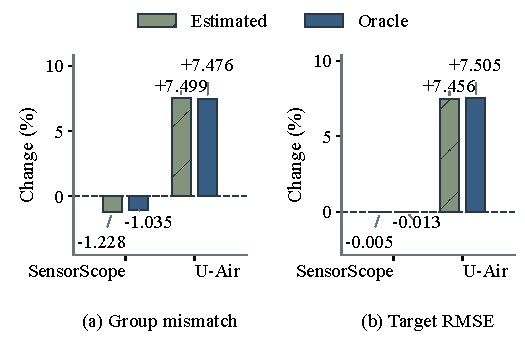
\includegraphics[width=\columnwidth]{fig_w1_design_gate.pdf}
\caption{Design sensitivity under estimated and oracle propensities.
(a)~Group mismatch; (b)~target RMSE. Bars show
$100(M_{\mathrm{Design}}-M_{\mathrm{NoDesign}})/M_{\mathrm{NoDesign}}$
over 20 seeds; positive means Design is worse.}
\label{fig:w1_design_gate}
\end{figure}

Against FedAU and ObsUse, respectively, SensorScope Design has TEST
worst-group RMSE changes of $-.01\%$ and $+.05\%$; U-Air NoDesign has
$+.48\%$ and $+.44\%$. Both meet the descriptive tolerance. The corresponding
all-20-seed changes are $+.02\%$ and $+.10\%$ on SensorScope, and $+.002\%$
and $+.075\%$ on U-Air. U-Air Design exceeds the tolerance, with changes of
$7.9\%$ and $8.0\%$ against the same comparators. The 20-seed Holm tests do
not establish prediction superiority. U-Air RAVEN improves worst-group RMSE
by $2.46\%$ over TwoStage-H\'ajek on TEST seeds within the Design-on family,
but its absolute RMSE of $1.2630$ remains above FedAvg's $1.1690$.


Under-served-block validation meets no-harm but misses the required improvement
against FedAU/ObsUse (Supplementary Table~\ref{tab:underserved_block};
\appref{app:underserved_block}). INT-R retains U-Air's Design trade-off,
while SensorScope's client--stratum advantage approaches zero (\appref{app:int_r}).
\label{subsec:eval_underserved}

\paragraph{Additional sensing protocols}
Real T-Drive opportunity is intermittent: active fraction $.425$, burstiness
$+.38$, and cell coverage $.547$.  Four-block opportunity--target TV is $.142$, compared with $.192$ on
SensorScope and $.278$ on U-Air under their respective protocols, all above $.05$
(Fig.~\ref{fig:g3_tdrive}; Table~\ref{tab:tdrive_hybrid}).
With controlled $O/U$, RAVEN-NoDesign fails the
$+.5\%$ worst-group tolerance: paired worst-group RMSE increases are $+2.39\%$ relative
to FedAU and $+2.43\%$ relative to ObsUse (versus FedAvg, $+.32\%$).  Its group gap equals FedAvg's;
Design on worsens prediction, worst-group risk, and group mismatch.  Delivery remains controlled.

\begin{figure}[t]
\raggedright
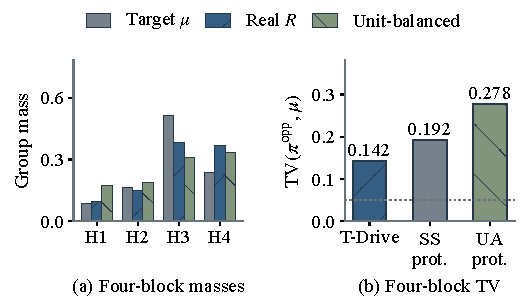
\includegraphics[width=\columnwidth]{fig_g3_tdrive_h_mass.pdf}
\caption{T-Drive opportunity and target mismatch.
(a)~Deployment target $\boldsymbol\mu$, real taxi $R$, and unit-balanced
reference. (b)~Four-block $\mathrm{TV}(\pi^{\mathrm{opp}},\boldsymbol\mu)$;
SS/UA denote the Complete-aligned SensorScope/U-Air protocols. The dotted $0.05$
line is the pre-specified mismatch-diagnostic threshold.}
\label{fig:g3_tdrive}
\end{figure}
\begin{table}[!htbp]
\centering
\caption{T-Drive comparison under real sensing opportunities.
Real taxi $R$, controlled $O/U$; mean $\pm$ SD over ten seeds; 178 windows;
lower is better. WorstGroupRMSE uses UTC H1--H4.
FedAvg, FedAU and ObsUse are Window variants.}
\label{tab:tdrive_hybrid}
\footnotesize
\setlength{\tabcolsep}{1pt}
\begin{tabular}{lcccc}
\toprule
Method & $\mathrm{RMSE}_{\mu}$ & \shortstack{WorstGroup\\RMSE} &
$\Delta_{\mathrm{group}}$ & $\Delta_{c\text{-}s}$\\
\midrule
FedAvg     & \shortstack{$1.1042$\\$\pm0.0022$} & \shortstack{$1.3064$\\$\pm0.0035$} & $0.5232$ & \shortstack{$1.9758$\\$\pm0.0004$}\\
TwoStage-H\'ajek    & \shortstack{$1.1254$\\$\pm0.0142$} & \shortstack{$1.3373$\\$\pm0.0198$} & \shortstack{$0.5948$\\$\pm0.0124$} & \shortstack{$1.9642$\\$\pm0.0007$}\\
FedAU      & \shortstack{$1.0898$\\$\pm0.0050$} & \shortstack{$1.2801$\\$\pm0.0109$} & $0.5232$ & \shortstack{$1.9915$\\$\pm0.0012$}\\
ObsUse     & \shortstack{$1.0896$\\$\pm0.0049$} & \shortstack{$1.2796$\\$\pm0.0108$} & $0.5232$ & \shortstack{$1.9916$\\$\pm0.0012$}\\
RAVEN-NoDesign & \shortstack{$1.1069$\\$\pm0.0028$} & \shortstack{$1.3106$\\$\pm0.0044$} & $0.5232$ & \shortstack{$1.9936$\\$\pm0.0003$}\\
RAVEN-Design & \shortstack{$1.1242$\\$\pm0.0159$} & \shortstack{$1.3355$\\$\pm0.0225$} & \shortstack{$0.5948$\\$\pm0.0124$} & \shortstack{$1.9774$\\$\pm0.0006$}\\
\bottomrule
\end{tabular}
\end{table}

The separate NSW four-region protocol ranking
(\appref{app:traffic_four_region}) favors TwoStage-H\'ajek on prediction
and worst-group RMSE and FedAU on group mismatch ($.0606$ versus RAVEN's
$.1048$); RAVEN stays within the descriptive worst-group tolerance against
FedAU/ObsUse under its local four-region target.

\paragraph{Target-risk and arrival-risk comparison}


The five-seed balanced control meets its $3\%$ no-harm margin: RAVEN versus
TimeAlign degrades by $.0599\%$, with one-sided 95\% upper bound $.134\%$ (\appref{app:e1_balanced}).
Under complete-aligned NSW-Traffic, define target and arrival changes from
balanced as $\Delta_\mu,\Delta_\rho$ and
$D_{\mathrm{aligned}}=\Delta_\mu-\Delta_\rho$.
Figure~\ref{fig:risk_noninterchangeability} gives mean $D$ from $-.0209$ to
$-.0214$, 17--18 negative seeds per method, and paired
$p=4.83\times10^{-4}$--$5.86\times10^{-4}$.  Target change is about
$8\times10^{-4}$ versus $2.2\times10^{-2}$ arrival change, showing that
selection affects the two risk views differently.
The six-scenario contrasts distinguish compounding and cancellation under
the constructed layers (\appref{app:e2_layer_matrix}).

\begin{figure}[t]
\raggedright
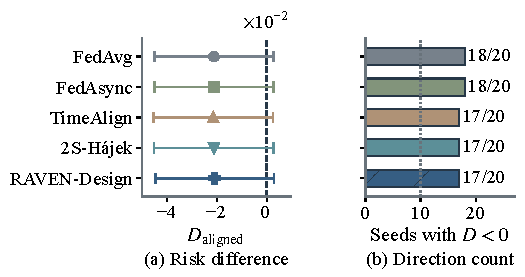
\includegraphics[width=\columnwidth]{fig2_e2_risk_noninterchangeability.pdf}
\caption{Target and arrival-risk changes on NSW-Traffic.
Complete-aligned selection: (a)~Mean points with $\pm$ sample-SD intervals over 20 paired seeds of
$D_{\mathrm{aligned}}=\Delta\mathrm{RMSE}_{\mu}-\Delta\mathrm{RMSE}_{\rho}$;
zero denotes equal changes. Negative $D$ means a larger arrival-risk change.
(b)~Negative-seed counts; dotted line: 10/20. Counts describe direction,
not significance or performance ranking.}
\label{fig:risk_noninterchangeability}
\end{figure}

Arrival-weighted validation shifts the reported risk by $-4.11\%$ to
$-4.12\%$ on SensorScope and $+.27\%$ to $+.62\%$ on U-Air, yet selects
the same configuration on all 20 seeds. In these comparisons, the scoring
distortion changes reported error more than configuration selection.



\subsection{Mechanism Contributions (RQ2)}
\label{subsec:rq2_mechanisms}
\label{subsec:eval_rq2}
\label{subsec:eval_rq3}

\paragraph{Matched-support comparison}
Table~\ref{tab:trained_rules} shares the Design-on correction pathway and
RAVEN's active support across count weighting, Uniform, reference projection,
Inst-Cal, and full RAVEN calibration.  Its U-Air count row is not the unrestricted FedAvg row
of Table~\ref{tab:main_effectiveness}.  The target and cap/ESS definitions are common, but Count is uncalibrated;
prediction follows the common saved-parameter scoring rule above.

\begin{table*}[t]
\centering
\caption{Trained aggregation rules on matched Design-on support.
Means over 20 paired seeds per dataset; lower is better.
Wall is wall-clock seconds per run. U-Air Count uses RAVEN-Design support,
unlike unrestricted FedAvg in Table~\ref{tab:main_effectiveness}.
}
\label{tab:trained_rules}
\footnotesize
\setlength{\tabcolsep}{5pt}
\begin{tabular*}{\textwidth}{@{\extracolsep{\fill}}llrrrrr}
\toprule
Dataset & Server-weight rule & $\Delta_{\mathrm{group}}$ & $\Delta_{c\text{-}s}$ &
$\mathrm{RMSE}_\mu$ & WorstGroupRMSE & Wall (s)\\
\midrule
SensorScope & Count / matched support & $1.05577$ & $1.29032$ & $7.93889$ & $8.67161$ & $20.5$\\
SensorScope & Uniform & $1.02693$ & $1.27069$ & $7.93931$ & $8.67202$ & $20.0$\\
SensorScope & Reference projection & $1.01158$ & $1.26903$ & $7.93725$ & $8.66989$ & $19.9$\\
SensorScope & Projection with debt ($\kappa=1000$) & $0.98464$ & $1.26659$ & $7.93842$ & $8.67109$ & $18.5$\\
SensorScope & Inst-Cal & $1.01409$ & $1.26443$ & $7.93799$ & $8.67066$ & $26.2$\\
SensorScope & Full RAVEN-Design & $1.01394$ & $1.26438$ & $7.93799$ & $8.67066$ & $27.1$\\
\midrule
U-Air & Count / matched support & $1.12176$ & $1.26213$ & $1.19225$ & $1.25956$ & $12.0$\\
U-Air & Uniform & $1.09734$ & $1.24065$ & $1.19349$ & $1.26094$ & $8.5$\\
U-Air & Reference projection & $1.09162$ & $1.23265$ & $1.19691$ & $1.26474$ & $8.8$\\
U-Air & Projection with debt ($\kappa=1000$) & $1.08001$ & $1.22623$ & $1.19470$ & $1.26231$ & $9.0$\\
U-Air & Inst-Cal & $1.09241$ & $1.23342$ & $1.19537$ & $1.26304$ & $15.1$\\
U-Air & Full RAVEN-Design & $1.09236$ & $1.23339$ & $1.19537$ & $1.26303$ & $15.3$\\
\bottomrule
\end{tabular*}
\end{table*}

\paragraph{Reference reconstruction and feasible calibration}
The corrected reference can violate the executable constraints.
Projection reduces its group mismatch by 1.188 percentage points on
SensorScope and 1.399 on U-Air. This fixed-support contrast isolates the
conversion from a reconstructed reference to a feasible allocation.

Relative to Uniform, reference projection improves group mismatch by
0.768 percentage points on SensorScope and 0.286 on U-Air. Only SensorScope
consistently meets the pre-specified 0.5-percentage-point practical threshold.
An independent, same-support Design-on/off comparison on SensorScope gives
0.922 percentage points; this is a separate contrast, not an additive gain.
U-Air's changing support prevents that comparison.
\appref{app:matched_support_contrasts} reports the 95\% confidence intervals
and tuning/report-seed results.

Full RAVEN calibration has different effects on group and client--stratum
alignment. On SensorScope, it has 0.118 percentage points more group mismatch
than projection ($p_{\mathrm{Holm}}=0.019$), but 0.232 percentage points less
client--stratum mismatch. U-Air's group contrast is not significant.
Table~\ref{tab:trained_rules} reports prediction and runtime: projection is
faster on both datasets, while prediction contrasts are not Holm-significant.

Uniform accounts for $68.96\%$ of SensorScope's matched count-to-RAVEN group
reduction: total 2.09 percentage points (95\% CI: 1.87--2.31), partitioned into $1.44$ pp
count-to-Uniform and $.65$ pp remaining. U-Air gives 1.47 percentage points
(95\% CI: 1.18--1.75), partitioned into $1.22$ pp ($83.07\%$) and $.25$ pp.
These mean-difference shares describe this shared pathway, not causal
component contributions or additive gains across the following comparisons.
The hindsight structural reference has a group-TV gap from Uniform of
$3.44$ pp on SensorScope and $1.32$ pp on U-Air over 20 always-on seeds. U-Air FedAU/ObsUse use
different supports and do not enter this attribution.

\paragraph{Component contributions}

Table~\ref{tab:e4_ablation} removes one component from Design-on under paired
Complete-aligned traces, not universally fixed active support, reporting
$100(M_{\mathrm{removed}}-M_{\mathrm{full}})/M_{\mathrm{full}}$.
The Design row includes the support changes described in
Section~\ref{subsec:rq1_alignment}, not the fixed-support projection intervention.
The Inst ablation removes instantaneous calibration, whereas Inst-Cal removes
debt. Removing instantaneous calibration worsens SensorScope client--stratum mismatch by $.310\%$.
On U-Air it worsens RMSE by $.143\%$ and tail RMSE by $.149\%$
($p_{\mathrm{Holm}}=.0194$), without significant structural changes.
Removing Obs significantly worsens U-Air group mismatch by $.123\%$ but
improves SensorScope client--stratum mismatch by $.070\%$. Removing Use has
no significant core effect after adjustment. Removing Debt significantly
increases group and client--stratum mismatch by $.0141\%$ and $.0040\%$ on
SensorScope, and by $.0043\%$ and $.0024\%$ on U-Air, respectively.
With the pre-specified debt coefficient, adding debt to projection changes
group-TV by $.0073$ pp on SensorScope and $.0024$ pp on U-Air. These
increments and the group, variance, and staleness effects lie inside the
registered practical band. The $\kappa=1000$ rule is a separate sensitivity
comparison.

\begin{table}[!htbp]
\centering
\caption{Component-removal effects.
Relative changes (\%) from full RAVEN: positive worsens, negative improves.
$^\ast$: Holm-adjusted $p<0.05$.}
\label{tab:e4_ablation}
\setlength{\tabcolsep}{3.5pt}
\begin{tabular}{llrrrr}
\toprule
Dataset & Removed & $\Delta_{\mathrm{group}}$ &
$\Delta_{c\text{-}s}$ & $\mathrm{RMSE}_{\mu}$ & Tail RMSE\\
\midrule
\multirow{5}{*}{SensorScope}
& Design & $+1.237^\ast$ & $+0.597^\ast$ & $+0.005$ & $+0.005$\\
& Obs    & $+0.096$       & $-0.070^\ast$ & $+0.012$ & $+0.011$\\
& Use    & $+0.026$       & $+0.026$       & $+0.012$ & $+0.012$\\
& Inst   & $-0.260$       & $+0.310^\ast$ & $-0.002$ & $-0.002$\\
& Debt   & $+0.014^\ast$ & $+0.004^\ast$ & $<0.001$ & $<0.001$\\
\midrule
\multirow{5}{*}{U-Air}
& Design & $-6.943^\ast$ & $+4.990^\ast$ & $-6.885^\ast$ & $-7.221^\ast$\\
& Obs    & $+0.123^\ast$ & $+0.022$       & $-0.010$       & $-0.010$\\
& Use    & $+0.014$       & $-0.014$       & $+0.025$       & $+0.026$\\
& Inst   & $-0.089$       & $-0.143$       & $+0.143^\ast$ & $+0.149^\ast$\\
& Debt   & $+0.004^\ast$ & $+0.002^\ast$ & $<0.001$ & $<0.001$\\
\bottomrule
\end{tabular}
\end{table}

Constant within-client weights cancel in local normalization, while corrected
client masses can still affect server weights in the original station blocks (\appref{app:local_hajek}).
The within-stratum heterogeneity experiment varies time-tercile covariates at fixed block observation means
(Supplementary Table~\ref{tab:f1_mechanism}; \appref{app:f1_mechanism}), providing within-stratum heterogeneous
inputs to the correction pathway.

Numerical endpoint and feasibility diagnostics:
\apprefs{app:kappa_probe}{app:p2_diagnostics}.

Component effects are endpoint-specific, with a small standard-strength debt
contribution and distinct alignment/runtime trade-offs.

\subsection{Target Support and Feasible Adjustment (RQ3)}
\label{subsec:rq3_adjustment}
\label{subsec:ceiling}

\paragraph{Support and constraint geometry}

With $E_{\min}=3$, $K_r\le3$ forces Uniform by the simplex norm bound.
In the Complete-aligned station protocol this covers $78.6\%$ of 1877 SensorScope windows,
$90.2\%$ of 1402 U-Air Design-on windows, and $79.0\%$ of 1515 Design-off
windows.  The largest target groups carry only $.53\%$ on SensorScope and $.79\%$ on U-Air.
Across 3279 evaluated active windows the feasible L1 group-distance range has
median $10^{-13}$; this does not make the squared L2 term in calibration constant.

For group range $W_{r,g}=\max_{\alpha\in\mathcal C_r}(M_r\alpha)_g-
\min_{\alpha\in\mathcal C_r}(M_r\alpha)_g$, adjustable target mass sums
$\mu_g$ where $W_{r,g}\ge.01$.
\appref{app:arrival_support} separates missing, narrow-range, and adjustable
target mass on nonempty arrival logs, distinct from complete calibration
support and cumulative service. Separate development cap/ESS scans appear in
\appref{app:development_geometry}.

\paragraph{Target-support variants}
\label{subsec:cityscanner_target_support}
Table~\ref{tab:cityscanner_sixarm} tests whether group-alignment gains persist
across target support and client--stratum shapes on ten shared visit-occupancy
traces, each with three model seeds. Floor fills the control map's zero masses
and renormalizes. M1$\mu$/M2$\mu$ use ACS population/NYC~311 shapes on the
same control keys, rescaled within region to the public $\boldsymbol\mu$.
These are trained target-map variants; \appref{app:cityscanner_sixarm}
gives their construction and statistical details.

\begin{table*}[t]
\centering
\caption{City Scanner visit-occupancy target-map variants.
Mean $\pm$ SD over ten trace means, each averaging three model seeds.
Predictions share region weights and a training-standardized scale.
$\rho$ is the percentage of non-test delivered units assigned zero mass
(zero with Design off). Group gaps use the common public region target;
bold marks endpoint minima.}
\label{tab:cityscanner_sixarm}
\footnotesize
\begin{tabular*}{\textwidth}{@{\extracolsep{\fill}}lrrrr@{}}
\toprule
Method / target map & $\rho$ (\%) & $\Delta_{\mathrm{group}}\downarrow$ &
$\mathrm{RMSE}_{\mu}\downarrow$ & WorstGroupRMSE $\downarrow$\\
\midrule
FedAvg / count & 0.00 & $0.1953{\pm}0.0342$ & $\mathbf{0.2409}{\pm}0.0832$ & $\mathbf{0.2529}{\pm}0.0903$\\
RAVEN-NoDesign & 0.00 & $0.0736{\pm}0.0264$ & $0.2439{\pm}0.0835$ & $0.2575{\pm}0.0905$\\
RAVEN-control & 14.35 & $0.0706{\pm}0.0266$ & $0.2561{\pm}0.1031$ & $0.2695{\pm}0.1095$\\
RAVEN-floor & 0.00 & $\mathbf{0.0682}{\pm}0.0313$ & $0.2442{\pm}0.0842$ & $0.2576{\pm}0.0908$\\
RAVEN-M1$\mu$ & 1.01 & $0.0771{\pm}0.0338$ & $0.2467{\pm}0.0889$ & $0.2609{\pm}0.0971$\\
RAVEN-M2$\mu$ & 0.98 & $0.0813{\pm}0.0301$ & $0.2508{\pm}0.0907$ & $0.2661{\pm}0.1003$\\
\bottomrule
\end{tabular*}
\end{table*}

Floor, M1$\mu$, and M2$\mu$ each reduce group mismatch versus FedAvg on
all ten paired traces and pass the three pre-specified structural comparisons
under the graphical multiplicity allocation (one-sided paired Wilcoxon,
each $p=9.77\times10^{-4}$). Floor retains $101.9\%$ of the FedAvg-to-control
group gain. The gains therefore remain observable in these support/shape
variants; NoDesign also has lower group mismatch than M1$\mu$/M2$\mu$.

Relative to FedAvg, the one-sided 95\% prediction upper bounds are $3.83\%$
for floor, $4.14\%$ for M1$\mu$, and $8.15\%$ for M2$\mu$. All exceed the
$2\%$ non-inferiority margin;
the gated superiority tests therefore remain untested. The control/floor paired prediction ratio remains inconclusive;
floor changes group marginals as well as zero masses. The graphical primary
chains and secondary Holm family retain separate identities
(\appref{app:cityscanner_sixarm}). Client--stratum targets are arm-specific
(Supplementary Table~\ref{tab:cityscanner_sixarm_cs}).

\paragraph{Reference sensitivity}
In the conditional perturbation analysis, stabilization error has median zero
but reaches $\ell_1$ maxima of $.553$ on SensorScope and $.680$ on U-Air (\appref{app:a5_a6_audit}). Replacing estimated margins
can change reference mass appreciably while prediction remains insensitive
(\appref{app:reference_sensitivity}).
Evaluated oracle configurations are sensitivity references, not predictive
optima. Concentrating the Traffic target raises the observed oracle contrast
to $.0970\%$, still below its $2\%$ practical criterion
(Supplementary Table~\ref{tab:target_concentration}; \appref{app:target_concentration}).
Formal station RMSE exceeds training-mean references
(\appref{app:formal_prediction_references}); separate development validation
improves on simple baselines on Traffic/SensorScope, not U-Air
(\appref{app:learning_capacity}).
Learning and update-rule budgets remain distinct
(\apprefs{app:learning_capacity}{app:update_rule_sensitivity}).

Support and constraints limit group-mass adjustment; feasible weight changes
need not change composition or prediction error.

\section{Conclusion}
\label{sec:conclusion}

RAVEN-MCS reconstructs a reference through sequential sensing-unit correction
and converts it into executable client mixtures under finite-window
constraints. Full RAVEN attains the lowest mean group mismatch among five
methods in each of two City Scanner protocols. Matched-support comparisons
identify the roles of count-weighting, reference correction, and calibration;
geometry shows where group mass can actually be adjusted. Ideal moment
recovery and fixed-window stability support reconstruction and calibration,
respectively, while long-run alignment additionally requires sublinear debt
growth. The evidence supports deployment-group alignment within the evaluated
support and constraints.

\section*{Acknowledgment}

OpenAI ChatGPT and Codex were used to assist with drafting and
revising portions of the Abstract, Sections I--VIII, and the
supplementary material. This assistance included organizing
technical explanations and refining language. These tools also
assisted in developing experimental implementation and plotting
code, and in designing and revising the workflow illustration
in Fig.~\ref{fig:raven_overview}. The authors take full
responsibility for the accuracy, integrity, and originality
of the manuscript, including the theoretical arguments,
experimental procedures, results, and citations.

\section*{Data and Code Availability}
The public sources are cited in Table~\ref{tab:datasets}.  T-Drive follows
Microsoft Research terms~\cite{yuan2010tdrive}.  City Scanner
{PM}$_{2.5}$~\cite{wang2023cityscanner} is Zenodo 10.5281/zenodo.7961851,
CC BY 4.0. Author-held materials include selection configurations, target maps,
event traces, City Scanner result summaries, and matched-support scoring inputs.
These materials are retained locally; no public access link is provided.

\FloatBarrier
\bibliographystyle{IEEEtran}
\bibliography{reference}

\begin{IEEEbiography}[{
\includegraphics[width=1in,height=1.25in,keepaspectratio]{authors/zuru_shi.jpg}}]{Zuru Shi}
is currently pursuing the bachelor's degree with the School of Computer
Science and Engineering, Central South University, Changsha, China.
Current research focuses on mobile crowdsensing, federated learning, and
spatiotemporal data completion, with an emphasis on selection bias,
deployment-target representation, and aggregation under finite-window
constraints.
\end{IEEEbiography}

\begin{IEEEbiography}[{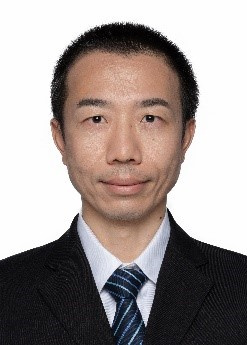
\includegraphics[width=1in,height=1.25in,keepaspectratio]{authors/tian_wang.jpg}}]{Tian Wang}
received the B.Sc. and M.Sc. degrees in computer science from Central South
University, Changsha, China, in 2004 and 2007, respectively, and the Ph.D.
degree in computer science from the City University of Hong Kong, Hong Kong,
in 2011. He is currently a Professor with the Institute of Artificial
Intelligence and Future Networks, Beijing Normal University, Zhuhai, China.
His research interests include the Internet of Things, edge computing, and
mobile computing.
\end{IEEEbiography}

\begin{IEEEbiography}[{
\includegraphics[width=1in,height=1.25in,keepaspectratio]{authors/houbing_song.jpg}}]{Houbing Herbert Song}
(Fellow, IEEE) received the Ph.D. degree in electrical engineering from the
University of Virginia, Charlottesville, VA, USA, in 2012. He is currently
a Professor with the Department of Information Systems, University of
Maryland, Baltimore County, Baltimore, MD, USA, where he directs the Security
and Optimization for Networked Globe Laboratory (SONG Lab).
\end{IEEEbiography}

\begin{IEEEbiography}[{
\includegraphics[width=1in,height=1.25in,keepaspectratio]{authors/anfeng_liu.jpg}}]{Anfeng Liu}
(Member, IEEE) is a Professor with the School of Electronic Information, Central South
University, Changsha, China. His research interests include wireless sensor
networks, mobile crowdsensing, and edge computing.
\end{IEEEbiography}

\vfill

\end{document}
